\documentclass[a4paper, 10pt]{report}

\usepackage{palatino}
%\usepackage{hyperref}
\usepackage{notes}

\usepackage{url}
%\usepackage{hyperref}
\usepackage{enumitem}
\usepackage{graphicx}
\usepackage{xspace}
%\usepackage{enumerate}
\usepackage{listings}
%\usepackage{draftwatermark}
\usepackage{fancyvrb}
\usepackage{lscape}
\usepackage{longtable}
\usepackage{fancyhdr}
\usepackage[nomessages]{fp}% http://ctan.org/pkg/fp
\usepackage{epsfig}
\usepackage{helvet}
\usepackage{color}
\usepackage{fancybox}
%\usepackage{enumerate}
\usepackage[hang, small, bf]{caption}
\usepackage{colortbl}
\usepackage{float}
\usepackage{amsmath}
\usepackage{amsfonts}
\usepackage[T1]{fontenc}
\usepackage{lmodern}
%\usepackage{type1cm}
\usepackage{relsize}


\usepackage[a4paper, top=3.5cm, bottom=3.5cm, left=2.5cm, right=2.5cm]{geometry}

\def\scalefactor{.95}
%\renewcommand\RSpercentTolerance{5}
\newcommand{\cn}[1]{{\sf\fontseries{sbc}\selectfont{\relscale{\scalefactor}#1}}}
\newcommand{\propertyname}[1]{{\sf\fontseries{sbc}\selectfont\relscale{\scalefactor}#1}}
\def\pmbexists{$\pmb\exists\:$\xspace}
\def\pmbforall{$\pmb\forall\:$\xspace}
\newcommand{\protege}{Prot\'eg\'e\xspace} 
\newcommand{\protegeowl}{Prot\'eg\'e 4\xspace} 
\newcommand{\todo}[1]{{\color{magenta}[TODO: #1]}}
%\newcommand{\ui}[1]{{\fontfamily{phv}\fontseries{m}\selectfont\small#1}}
\newcommand{\ui}[1]{{\sf\relscale{\scalefactor}#1}}
\def\typing#1{\texttt{#1}}

\definecolor{lightgray}{gray}{0.9}

\setlength{\fboxsep}{10pt}
\setlength{\parskip}{12pt}
\setlength{\parindent}{0pt}

\def\uiAddIcon{\ui{Add} icon~(\raise-2.5pt\hbox{\includegraphics[width=12pt]{images/png/PlusIcon.png}})\xspace}
\long\def\ignore#1{}

\newcommand{\largefigwidth}{16cm}
\newcommand{\medfigwidth}{12cm}
\newcommand{\figwidth}{8cm}
\makeatletter
\def\maxwidth{%
  \ifdim
    \Gin@nat@width>\figwidth
    \figwidth
  \else
    \Gin@nat@width
  \fi
}
\makeatother


\newcounter{stepscounter}

\newcommand{\steps}[2]{{
\vspace*{12pt}
\setlength{\tabcolsep}{0pt}
\begin{figure}[H]
\begin{center}
\begin{tabular}{l>{\columncolor[gray]{.75}}rcl}
\multicolumn{4}{l}{
\addtocounter{stepscounter}{1}
\textbf{\textsf{Task \arabic{stepscounter}:}}
\begin{minipage}[t]{14cm}
\textbf{\textsf{#1}}
\vspace{5pt}
\end{minipage}
} \\
 \hline
\\
  \hspace*{0pt} &
  \hspace*{8pt} &
  \hspace*{10pt}&
  \begin{minipage}[t]{14cm}
  \begin{enumerate}
#2
\end{enumerate}
 \end{minipage}\\\\
 \hline
\end{tabular}
\end{center}
\end{figure}
%\vspace*{12pt}
}}


\newcommand{\iconbox}[2]
{{
\begin{tabular}{ll}
\begin{minipage}{1.5cm}
\includegraphics{#1}
\end{minipage}

 &

\fbox{
\begin{minipage}[t]{12.5cm}
#2
\end{minipage}
}
\end{tabular}
\vspace*{12pt}
}}


\newcommand{\tip}[1]
{{
\iconbox{images/pdf/TipIcon.pdf}{#1}
}}

\newcommand{\meaningOf}[1]
{{
\iconbox{images/pdf/WhatDoesItMeanIcon.pdf}{#1}
}}

\newcommand{\warning}[1]
{{
\iconbox{images/WarningIcon.pdf}{#1}
}}

\newcommand{\dragon}[1]
{{
\iconbox{figures/dragon}{#1}
}}
\newcommand{\snapshot}[1]
{{
\iconbox{images/black_camera}{#1}
}}
\newcommand{\note}[1]
{{
\iconbox{images/NoteIcon.pdf}{#1}
}}

\newcommand{\vocab}[1]
{{
\iconbox{images/pdf/VocabIcon.pdf}{#1}
}}

\newcommand{\owlcode}[1]
{{
\iconbox{images/code.PNG}{#1}
}}

\newcommand{\expressivity}[1]
{{
\iconbox{images/NoteIcon.pdf}{The \fhkb ontology at this stage of the tutorial has an expressivity of $\mathcal{#1}$.}
}}
\newcommand{\ctime}[3]
{{
 \FPeval{\resulthermit}{round(#1/1000,3)}
 \FPeval{\resulthermitfrac}{round(#1/1891157,5)}
  \FPeval{\resultpellet}{round(#2/1000,3)}
 \FPeval{\resultpelletfrac}{round(#2/123655,5)}
  \FPeval{\resultfact}{round(#3/1000,3)}
 \FPeval{\resultfactfrac}{round(#3/35438,3)}
\iconbox{images/NoteIcon.pdf}{The time to reason with the FHKB at this point (in \protege) on a typical desktop machine by HermiT 1.3.8 is approximately \resulthermit\xspace sec ({\resulthermitfrac} \% of final), by Pellet 2.2.0 \resultpellet\xspace sec ({\resultpelletfrac} \% of final) and by FaCT++ 1.6.4 is approximately \resultfact\xspace sec ({\resultfactfrac} \% of final). 0 sec indicates failure or timeout.}
}}


\newcommand{\curex}
{{
	Exercise~\arabic{stepscounter}
}}

%%\pagestyle{fancy}

\newcommand{\authorlist}{Robert Stevens, Margaret Stevens, Nicolas Matentzoglu and Simon Jupp\xspace}
\newcommand{\fhkbhome}{\url{http://owl.cs.manchester.ac.uk/tutorials/fhkbtutorial}\xspace}

\newcommand{\comment}[1]{\textbf{\large #1}\xspace}
%\newcommand{\herebedragons}{{here be dragons}}
\newcommand{\herebedragons}{\marginpar{
\includegraphics[width=1cm]{figures/dragon}}}
\newcommand{\dragtext}[1]{\emph{#1}\marginpar{
\includegraphics[width=1cm]{figures/dragon}}}

\newcommand{\con}[1]{{\sf #1}\xspace}
%\newcommand{\comment}[1]{\textbf{\large #1}\xspace}
%\newcommand{\todo}[1]{\textbf{\large #1}\xspace}
%\newcommand{\protege}{Prot\'eg\'e\xspace}
\newcommand{\fhkb}{FHKB\xspace}
\newcommand{\indiv}{individual\xspace}

\newcommand{\rds}{Robert David Bright\xspace}
\newcommand{\ds}{David Bright\xspace}
\newcommand{\mgs}{Margaret Grace Rever\xspace}
\newcommand{\rjs}{Richard John Bright\xspace}


\newcommand{\irds}{\con{Robert\_David\_Bright\_1965}\xspace}
\newcommand{\irjs}{\con{Richard\_John\_Bright\_1962}\xspace}
\newcommand{\imgs}{\con{Margaret\_Grace\_Rever\_1934}\xspace}
\newcommand{\iwgs}{\con{William\_George\_Bright\_1901}\xspace}
\newcommand{\ids}{\con{David\_Bright\_1934}\xspace}
\newcommand{\iiea}{\con{Iris\_Ellen\_Archer\_1907}\xspace}
\newcommand{\ijb}{\con{John\_Bright\_1930}\xspace}
\newcommand{\ipwb}{\con{Peter\_William\_Bright\_1941}\xspace}

\newcommand{\stevens}{Stevens\xspace}
\newcommand{\person}{\con{Person}}
\newcommand{\female}{\con{Femaleness}}
\newcommand{\male}{\con{Maleness}}
\newcommand{\sex}{\con{Sex}}
\newcommand{\woman}{\con{Woman}}
\newcommand{\man}{\con{Man}}
\newcommand{\owlii}{OWL~2\xspace}

\newlist{tasks}{enumerate}{1}
\newcommand{\taskstart}{\setlist[tasks]{label=\emph{\thechapter.\arabic*}}}
\newcommand{\taskcont}{\setlist[tasks]{resume,label=\emph{\thechapter.\arabic*}}}


%\lstnewenvironment{owlcode} {\small} {}{#1}}




\title{\sc{Manchester Family History Advanced OWL Tutorial\\Edition 1.1}}
\author{\\\authorlist\\\\
Bio-Health Informatics Group\\
School of Computer Science\\
University of Manchester\\
Oxford Road\\
Manchester\\
United Kingdom\\
M13 9PL\\
\\
\url{robert.stevens@manchester.ac.uk}
\\
\\
\\
\textbf{Contributors}\\[6pt]
{\def\v{v\hskip2pt}
\def\arraystretch{1.3}
\begin{tabular}{rl}
\v 1.0&\authorlist\\
\v 1.1&Robert Stevens, Nicolas Matentzoglu\\
\end{tabular}
}
\\
\vspace{90pt}
\\
\small{\textsc{The University of Manchester}}\\[10pt] 
%\\
%\\
%\\
Copyright $\copyright$ ~The University of Manchester
}


\begin{document}
\maketitle

\pagenumbering{roman}

\section*{Acknowledgements}

This tutorial was realised as part of the Semantic Web Authoring Tool (SWAT) project (see \url{http://www.swatproject.org}), which is supported by the UK Engineering and Physical Sciences Research Council (EPSRC) grant EP/G032459/1, to the University of Manchester, the University of Sussex and the Open University.


\section*{Dedication}

The Stevens family---all my ancestors were necessary for this to happen. Also, for my Mum who gathered all the information.

\tableofcontents
%\listoffigures
%\listoftables


\chapter*{Preamble}

\section{Licencing}

The `Manchester Family History Advanced OWL Tutorial' by Robert Stevens, Margaret Stevens, Nicolas Matentzoglu, Simon Jupp is licensed under a Creative Commons
Attribution-ShareAlike 3.0 Unported License.\marginpar{
\includegraphics[width=1cm]{figures/licence_logo}}


\section{Reporting  Errors}

This manual will almost certainly contain errors, defects and infelicities. Do report them to \url{robert.stevens@manchester.ac.uk}. Supplying chapter, section and some actual context in the form of words will help in fixing any of these issues.

\section{Acknowledgements}

As well as the author list, many people have contributed to this work. Any contribution, such as reporting bugs etc., is rewarded by an acknowledgement of contribution (in alphabetical order) when the authors get around to adding them:

\begin{itemize}
\item Graham Goff;
\item Matthew Horridge;
\item Jared Leo;
\item Fennie Liang;
\item Phil Lord;
\item Fiona McNeill;
\item Eleni Mikroyannidi; 
\item George Moulton;
\item Bijan Parsia;
\item Alan Rector;
\item Uli Sattler;
%\item Margaret Stevens;
\item Dmitry Tsarkov;
\item Danielle Welter.
\end{itemize}
\cleardoublepage
\addcontentsline{toc}{chapter}{Preamble}

\pagenumbering{arabic}

\chapter{Introduction}


These exercises in the Web Ontology Language (OWL) take participants through OWL from its basics to some rather advanced features of the OWL~DL profile of OWL. The exercises use family history as a topic and much of the tutorial is based on the `Manchester Family History Advanced OWL Tutorial' found at \url{http://owl.cs.manchester.ac.uk/publications/talks-and-tutorials/fhkbtutorial/}. Here, instead of an `advanced tutorial', the exercises go from the start to quite a lot of what anyone using OWL to model needs to know about the language and the use of an automated reasoner; the exercises do not really explore much in the way of modelling issues.	 

These exercises don't give any instruction in \protege; for that use the Pizza tutorial at \url{http://owl.cs.manchester.ac.uk/tutorials/protegeowltutorial/}. These exercises don't give any explanation behind the phenomena revealed during the exercises; these are explained by the human beings delivering the exercises. More explanation can be found in the Pizza tutorial and the written, original, long version of the Family History OWL tutorial is in Blackboard.

In these exercises we take an ``objects (individuals) first'' approach. Most tutorials concentrate on classes then individuals (if at all). By doing it this way our aim is to emphasise  that OWL is all about modelling individuals--even if most axioms are restrictions upon classes that say `each and every individual in this class holds at least one of these properties to an individual of the filler class'. Similarly, object properties are relationships between two individuals, we just usually model at the class level and these sort of distinctions can sometimes get lost. So, these exercises start with asserting lots of properties between named individuals and only later do we start talking about classes of these individuals. It may be, and probably will be, that most modelling is with classes and properties, but this way really emphasises what the language is actually doing.

Subsequent material in the course unit will focus largely on classes and modelling with classes. 

Once you have completed these exercises in the lab, you are recommended to work your way through the Protege Pizza tutorial and the Family History OWL Tutorial. These will help you gain experience of the mechanics of using \protege and provide a further introduction to \owlii. 

\begin{itemize}
\item \url{http://owl.cs.manchester.ac.uk/tutorials/protg-owl-tutorial/}
\item \url{http://owl.cs.manchester.ac.uk/publications/talks-and-tutorials/fhkbtutorial/} contains the ontologies, and the long version of the tutorial explanation is in Blackboard. 
\end{itemize}

\section{Learning outcomes}

By the end of a successful completion of these exercises you should be able to:

\begin{enumerate}
\item Understand the core aspects of \owlii syntax and semantics;
\item Use \protege to build an ontology, and use an automated reasoner to draw inferences from the axioms in your ontology;
\item Use classes and individuals;
\item Use \owlii's property hierarchy;
\item Use \owlii's property characteristics;
\item Know more than you need to about the famly history of \rds;
\item Know some of the limitations of \owlii.
\end{enumerate}
\noindent These learning outcomes are very generic; each exercise encapsulates a significant learning outcome. For example, Exercise~\ref{ex:date} has a learning outcome of: knowing how to use data properties; knowing about and using the \con{DifferentIndividuals} axiom; a reinforcement of the use of the functional property characteristic; and an introduction to qualified cardinality restrictions.

\section{Assumptions}


We make some simplifying assumptions in this tutorial:
\begin{itemize}
\item We assume people doing the exercises know nothing about OWL.
\item We assume that there are human beings present that are knowledgeable about OWL to conduct participants through the exercises and give explanations. You may need to ask these human beings (or consult some other sources) to understand some of the terms used in this tutorial (e.g., ``inverse'' or ``transitive''). 
\item We take a conventional western  view of family history. This appears to have most effects on naming of sibling and cousin relationships.
\item We take a straight-forward view on the sex of people; this is explored further in Chapter~\ref{ex:sex};
%\item A 'conventional' view of marriage is taken; this is explored further in Chapter~\ref{chap:marriage}.
\item We make no special treatment of time or dates; we are only interested in years and we do not do anything fancy; this is explored more in Chapter~\ref{ex:date}.
\end{itemize}
At the end of the tutorial, you should be able to produce a property hierarchy and a TBox or class hierarchy; all supported by use of \protege, the automated reasoner, and a lot of \owlii's features.

% At the end of the tutorial, you should be able to produce a property hierarchy and a TBox or class hierarchy  such as shown in Figure~\ref{fig:class_and_prop_hierachy}; all supported by use of the automated reasoner and a lot of \owlii's features.

% \begin{figure}
% \begin{center}
% 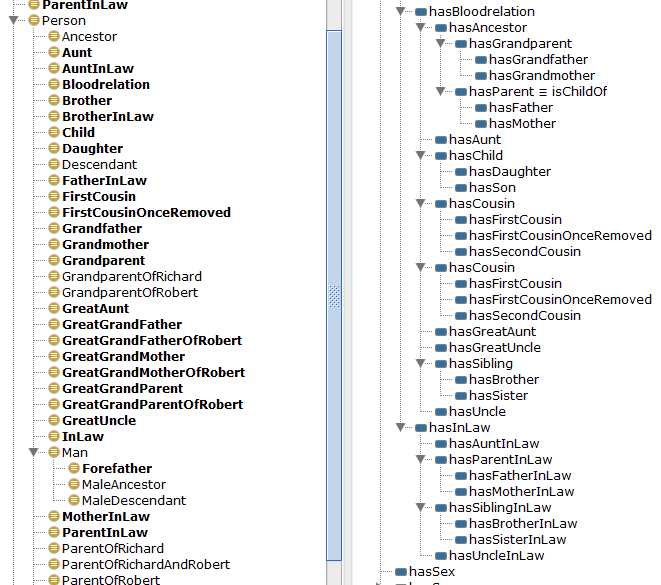
\includegraphics[width=\largefigwidth]{figures/class_prop_hierachy_final}\caption{A part of the class and property hierarchy of the final \fhkb.}\label{fig:class_and_prop_hierachy}
% \end{center}
% \end{figure}


\section{How to use these exercises}

Start at exercise one and work through to the last exercise. Don't just read the exercises and think you know what will happen; actually do it and you'll learn more. 
\chapter{Adding some Individuals to the \fhkb}
\label{chap:indiv}

In this chapter we will start by creating a fresh OWL ontology and adding some individuals that will be surrogates for people in the \fhkb. In particular you will:

\begin{enumerate}
\item Create a new OWL ontology for the \fhkb;
\item Add some individuals that will stand for members of the \stevens family.
%of the class \con{Person};
%\item Assert them to be members of the class \con{Person};
\item Describe parentage of people.
\item Add some facts to specific individuals as to their parentage;
\item See the reasoner doing some work.
\item At the moment we will ignore sex; sex will not happen until Chapter~\ref{chap:person}.
\end{enumerate}

\section{A World of Objects}

The `world'\footnote{we use `world' as a synonym of `field of interest' or `domain'. `World' does not restrict us to modelling the physical world outside our consciousness. } or field of interest we model in an ontology is made up of objects or individuals. Such objects include, but are not limited to:
\begin{itemize}
\item People, their pets, the pizzas they eat;
\item The processes of cooking pizzas, living, running, jumping, undertaking a journey;
\item The spaces within a room, a bowl, an artery;
\item The attributes of things such as colour, dimensions, speed, shape of various objects;
\item Boundaries, love, ideas, plans, hypotheses.
\end{itemize}
\noindent We observe these objects, either outside lying around in the world or in our heads. OWL is all about modelling such individuals. Whenever we make a statement in OWL, when we write down an axiom, we are making statements about individuals. When thinking about the axioms in an ontology it is best to think about the individuals involved, even if OWL individuals do not actually appear in the ontology. All through this tutorial we will always be returning to the individuals being described in order to help us understand what we are doing and to help us make decisions about how to do it.

\section{Asserting Parentage Facts}

%So far, through the description of the \person class, we know that all instances of the class \person have a mother and father; we  have seen this through the use of a DL query. We do not, however, know about the actual parents of people in the \fhkb.

%So far, we have done assertion of types on individuals; now we come to fact assertions. 

Biologically, everyone has parents; a mother and a father\footnote{Don't quibble; it's true enough here.}. The starting point for family history is parentage; we need to relate the family member objects by object properties. An object property relates two objects, in this case a child object with his or her mother or father object. To do this we need to create three object properties:

\steps{Creating object properties for parentage}{
\item Create a new ontology;
\item Create an object property \con{hasMother}; 
\item Create a property \con{isMotherOf} and give \con{hasMother} the \texttt{InverseOf:} \con{isMotherOf};
\item Do the same for the property \con{hasFather};
\item Create a property \con{hasParent}; give it the obvious inverse;
\item Make \con{hasMother} and \con{hasFather} sub-properties of \con{hasParent}.
\item Run the reasoner and look at the property hierarchy.
}

Note how the reasoner has automatically completed the sub-hierarchy for \con{isParentOf}: \con{isMotherOf} and \con{isFatherOf} are inferred to be sub-properties of \con{isParentOf}. 

The OWL snippet below shows some parentage fact assertions on an individual. Note that rather than being assertions to an anonymous individual via some class, we are giving an assertion to a named individual. 
%Of course, we have asserted parentage `anonymously' at  the class level -- as a \emph{universal} statement about each and every instance of the class \person having a mother and a father.
\\\\
\owlcode{
Individual: grant\_plinth

	Facts:
		hasFather mr\_plinth,
		hasMother mrs\_plinth
}

\steps{Create the ABox}{
%\item Go back to the \con{fhkb.owl} (the state of the \fhkb at the end of the last chapter). 
\item Using the information in Table~\ref{tab:familydata} (see appendix) about parentage (so the columns about fathers and mothers), enter the fact assertions for the people which appear in rows shaded in grey. We will only use the \con{hasMother} and \con{hasFather} properties in our fact assertions. You do not need to assert names and birth years yet. This exercise will require you to create an individual for every person we want to talk about, using the Firstname\_Secondname\_Familyname\_Birthyear pattern, as for example in \irds. 
}


\snapshot{While asserting facts about all individuals in the \fhkb will be a bit tedious at times, it might be useful to at least do the task for a subset of the family members. For the impatient reader, there is a convenience snapshot of the ontology including the raw individuals available at \fhkbhome.}

\note{If you are working with \protege, you may want to look at the Matrix plugin for \protege at this point. The plugin allows you to add individuals quickly in the form of a regular table, and can significantly reduce the effort of adding any type of entity to the ontology. In order to install the matrix plugin, open \protege and go to File >> Check for plugins. Select the `Matrix Views' plugin. Click install, wait until the the installation is confirmed, close and re-open \protege; go to the `Window' menu item, select `Tabs' and add the `Individuals matrix'.}

Now do the following:
\steps{DL queries}{
\item Classify the \fhkb.
\item Issue the DL query \con{hasFather value \ids} and look at the answers (remember to check the respective checkbox in \protege to include individuals in your query results).
\item Issue the DL query \con{isFatherOf value \irds}. Look at the answers.
\item Look at the entailed facts on \irds.
}

You should find the following:
\begin{itemize}
\item David Bright (1934) is the father of Robert David Bright (1965) and Richard John Bright (1962).
\item Robert David Bright (1965)  has David Bright 1934 as a parent.
\end{itemize}

Since we have said that \con{isFatherOf} has an inverse of \con{hasFather}, and we have asserted that \irds \con{hasFather} \ids{}, we have a simple entailment that \ids \con{isFatherOf} \irds{}. So, without asserting the \con{isFatherOf} facts, we have been able to ask and get answers for that DL query.

As we asserted that \irds \con{hasFather} \ids{}, we also infer that he \con{hasParent} \ids{}; this is because \con{hasParent} is the super-property of \con{hasFather} and the sub-property implies the super-property. This works all the way up the property tree until \con{topObjectProperty}, so all individuals are related by \con{topObjectProperty}---this is always true. This implication `upwards' is the way to interpret how the property hierarchies work. 

%\section{Should I say it Just Because It's True?}

\section{Summary}
We have now covered the basics of dealing with individuals in OWL ontologies. We have set up some properties, but without domains, ranges, appropriate characteristics and then arranged them in a hierarchy. From only a few assertions in our \fhkb, we can already infer many facts about an individual: Simple exploitation of inverses of properties and super-properties of the asserted properties.

We have also encountered some important principles:
\begin{itemize}
\item We get inverses for free.
\item The sub-property implies the super-property. So, \con{hasFather} implies the \con{hasParent} fact between individuals. This entailment of the super-property is very important and will drive much of the  inference we do with the \fhkb.
\item Upon reasoning we get the inverses of properties between named individuals for free.
\item Lots is still open. For example, we do not know the sex of individuals and what other children, other than those described, people in the \fhkb may have.
\end{itemize}

\expressivity{ALHI}

\ctime{26}{144}{7}
\chapter{Ancestors and Descendants}
\label{chap:ancestor}
In this Chapter you will:
\begin{enumerate}
\item Use sub-properties and the transitive property characteristic to infer ancestors of people;
\item Add properties to the \fhkb property hierarchy that will infer ancestors and descendants of a person without adding any more facts to the \fhkb;
\item Explore the use of sub-property chains for grandparents, great grandparents and so on;
\item Place all of these new object properties in the property hierarchy and in that way learn more about the implications of the property hierarchy.
\end{enumerate}

\snapshot{Find a snapshot of the ontology at this stage at \fhkbhome.}

\section{Ancestors and Descendants}

The \fhkb has parents established between individuals and we know that all people have two parents. A parent is an ancestor of its children; a person's parent's parents are its ancestors; and so on. So, in our \fhkb, Robert's ancestors are David, Margaret, William, Iris, Charles, Violet, James, another Violet, another William, Sarah and so on. If my parent's parents are my ancestors, then what we need is a transitive version of the \con{hasParent} property. Obviously we do not want \con{hasParent} to be transitive, as Robert's grandparents (and so on) would become his parents (and that would be wrong).

We can easily achieve what is necessary. We need a \con{hasAncestor} property that has a transitive characteristic. The trick is to make this a super-property of the \con{hasParent} property. As explained before, a sub-property implies its super-property. So, if \indiv \emph{x} holds a \con{hasParent} property with an \indiv \emph{y}, then it also holds an instance of its super-property \con{hasAncestor} with the \indiv \emph{y}. If \indiv \emph{y} then holds a \con{hasParent} property with another \indiv \emph{z}, then there is also, by implication, a \con{hasAncestor} property between \emph{y} and \emph{z}. As \con{hasAncestor} is transitive, \emph{x} and \emph{z} also hold a \con{hasAncestor} relationship between them.

The inverse of \con{hasAncestor} can either be \con{isAncestorOf} or \con{hasDescendant}. We choose the \con{isAncestorOf} option.

\steps{Object properties: exploiting the semantics}{
\item Make a new object property \con{hasRelation}, make it symmetric.
\item Make a new object property \con{hasAncestor}.
\item Make it a sub-property of \con{hasRelation} and a super-property of \con{hasParent}.
\item Make \con{hasAncestor} transitive.
\item Create the inverse \con{isAncestorOf}. Do not `stitch' it into the property hierarchy; the reasoner will sort it all out for you.
\item Run the reasoner and issue the DL query \con{hasAncestor value \iwgs}.
\item Issue the query \con{isAncestorOf value \irds}.
}

The \con{hasAncestor} object property will look like this:

\owlcode{
ObjectProperty: hasAncestor

    SubPropertyOf: 
        hasRelation

    SuperPropertyOf: 
        hasParent,

    Characteristics: 
        Transitive

    InverseOf: 
        isAncestorOf
}\\\\
As usual, it is best to think of the objects or individuals involved in the relationships. Consider the three individuals -- Robert, David and William. Each has a \con{hasFather} property, linking Robert to David and then David to William. As \con{hasFather} implies its super-property \con{hasParent}, Robert also has a \con{hasParent} property with David, and David has a \con{hasParent} relation to William. Similarly, as \con{hasParent} implies \con{hasAncestor}, the Robert object has a \con{hasAncestor} relation to the David object and the David object has one to the William object. As \con{hasAncestor} is transitive, Robert not only holds this property to the David object, but also to the William object (and so on back through Robert's ancestors).

\section{Grandparents and Great Grandparents}

We also want to use a sort of restricted transitivity in order to infer grandparents, great grandparents and so on. My grandparents are my parent's parents; my grandfathers are my parent's fathers. My great grandparents are my parent's parent's parents. My great grandmothers are my parent's parent's mothers. This is sort of like transitivity, but we want to make the paths only a certain length and, in the case of grandfathers, we want to move along two relationships -- \con{hasParent} and then \con{hasFather}.

We can do this with \owlii's sub-property chains. The way to think about sub-property chains is: If we see property \emph{x} followed by property \emph{y} linking three objects, then it implies that property \emph{z} is held between the first and third objects. Figure~\ref{fig:chain_triangle} shows this diagrammatically for the hasGrandfather property.

\begin{figure}
\begin{center}
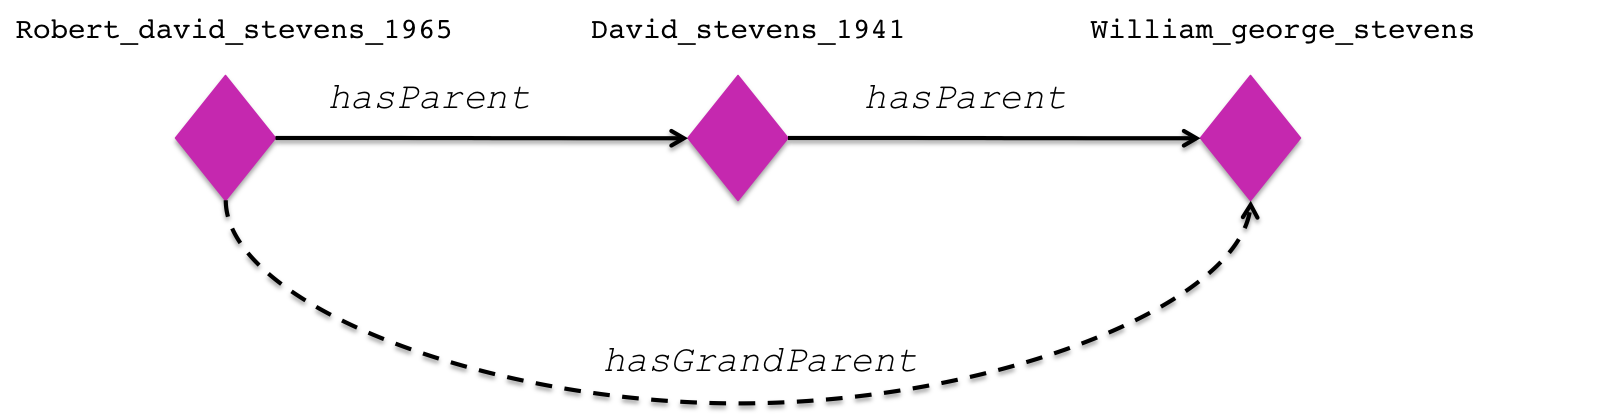
\includegraphics[width=\figwidth]{figures/grandparent}\caption{Three blobs representing objects of the class \person. The three objects are linked by a \con{hasParent} property and this implies a \con{hasGrandparent} property.}\label{fig:chain_triangle}
\end{center}
\end{figure}

For various grandparent object properties we need the following sets of implications:
\begin{itemize}
\item My parent's parents are my grandparents;
\item My parent's fathers are my grandfathers;
\item My parent's mothers are my grandmothers;
\item My parent's parent's parents are my great grandparents or my grandparent's parents are my great grandparents.
\item My parent's parent's fathers are my great grandfathers or my parent's grandfathers are my great grandfathers;
\item My parent's parent's mothers are my great grandmothers (and so on).
\end{itemize}

Notice that we can trace the paths in several ways, some have more steps than others, though the shorter paths themselves employ paths. Tracing these paths is what \owlii's sub-property chains achieve. For the new object property \con{hasGrandparent} we write:
\\\\
\owlcode{
ObjectProperty: hasGrandparent
SubPropertyChain:
hasParent o hasParent
}
\\\\
We read this as `\con{hasParent} followed by \con{hasParent} implies \con{hasGrandparent}'.
We also need to think where the \con{hasGrandparent} property fits in our growing hierarchy of object properties. Think about the implications: Does holding a \con{hasParent} property between two objects imply that they also hold a \con{hasGrandparent} property? Of course the answer is `no'. So, this new property is not a super-property of \con{hasParent}. Does the holding of a \con{hasGrandparent} property between two objects imply that they also hold an \con{hasAncestor} property? The answer is `yes'; so that should be a super-property of \con{hasGrandparent}. We need to ask such questions of our existing properties to work out where we put it in the object property hierarchy. At the moment, our \con{hasGrandparent} property will look like this:
\\\\
\owlcode{
ObjectProperty: hasGrandParent

    SubPropertyOf: 
        hasAncestor
    
    SubPropertyChain:
		hasParent o hasParent

    SuperPropertyOf: 
        hasGrandmother,
        hasGrandfather


    InverseOf: 
        isGrandParentOf
}
\\
Do the following task:
\steps{Grandparents object properties}{
\item Make the \con{hasGrandparent}, \con{hasGrandmother} and \con{hasGrandfather} object properties and the obvious inverses (see OWL code above);
\item Go to the individuals tabs and inspects the inferred object property assertions for \irds and his parents.
}

Again, think of the objects involved. We can take the same three objects as before: Robert, David and William. Think about the properties that exist, both by assertion and implication, between these objects. We have asserted only \con{hasFather} between these objects. The inverse can be inferred between the actual individuals (remember that this is not the case for class level restrictions -- that all instances of a class hold a property does not mean that the filler objects at the other end hold the inverse; the quantification on the restriction tells us this). Remember that:
\begin{enumerate}
\item Robert holds a \con{hasFather} property with David;
\item David holds a \con{hasFather} property with William;
\item By implication through the \con{hasParent} super-property of \con{hasFather}, Robert holds a \con{hasParent} property with David, and the latter holds one with William;
\item The sub-property chain on \con{hasGrandfather} then implies that Robert holds a \con{hasGrandfather} property to William. Use the diagram in figure~\ref{fig:chain_triangle} to trace the path; there is a \con{hasParent} path from Robert to William via David and this implies the \con{hasGrandfather} property between Robert and William.
\end{enumerate}

It is also useful to point out that the inverse of \con{hasGrandfather} also has the implication of the sub-property chain of the inverses of \con{hasParent}. That is, three objects linked by a path of two \con{isParentOf} properties implies that an \con{isGrandfatherOf} property is established between the first and third object, in this case William and Robert. As the inverses of \con{hasFather} are established by the reasoner, all the inverse implications also hold.

\section{Summary}

It is important when dealing with property hierarchies to think in terms of properties between objects and of the implications `up the hierarchy'. A sub-property implies its super-property. So, in our \fhkb, two person objects holding a \con{hasParent} property between them, by implication also hold an \con{hasAncestor} property between them. In turn, \con{hasAncestor} has a super-property \con{hasRelation} and the two objects in question also hold, by implication, this property between them as well.

We made \con{hasAncestor} transitive. This means that my ancestor's ancestors are also my ancestors. That a sub-property is transitive does not imply that its super-property is transitive. We have seen that by manipulating the property hierarchy we can generate a lot of inferences without adding any more facts to the individuals in the \fhkb. This will be a feature of the whole process -- keep the work to the minimum (well, almost).

In \owlii, we can also trace `paths' around objects. Again, think of the objects involved in the path of properties that link objects together. We have done simple paths so far -- Robert linked to David via \con{hasParent} and David linked to William via \con{hasFather} implies the link between Robert and William of \con{hasGrandfather}. If this is true for all cases (for which you have to use your domain knowledge), one can capture this implication in the property hierarchy. Again, we are making our work easier by adding no new explicit facts, but making use of the implication that the reasoner works out for us.

\expressivity{ALRI+}

\ctime{262}{30}{4}
\chapter{Modelling the \con{Person} Class}
\label{chap:person}
\taskstart 

In this Chapter you will:
\begin{enumerate}
%\item Create a basic ontology for the \fhkb;
\item Create a \con{Person} class;
\item Describe \con{Sex} classes;
\item Define \con{Man} and \con{Woman};
\item Ask which of the people in the \fhkb has a father.
\item Add domains and ranges to the properties in the \fhkb.
\item Make the \fhkb inconsistent.
\item  Add some more defined classes about people and see some equivalence  inferred between classes.
\end{enumerate}
These simple classes will form the structure for the whole \fhkb.


\section{The Class of Person}

For the \fhkb, we start by thinking about the objects involved
\begin{enumerate}
\item The people in a family -- Robert, Richard, David, Margaret, William, Iris, Charles, Violet, Eileen, John and Peter;
\item The sex of each of those people;
\item The marriages in which they participated;
\item The locations of their births;
\item And many more\ldots
\end{enumerate}

There is a class of \con{Person} that we will use to represent all these people objects.

\steps{Create the \con{Person} class}{
\item Create a class called \con{DomainEntity};
\item Create a subclass of \con{DomainEntity} called \con{Person}.
}
%\taskcont
\noindent We use \con{DomainEntity} as a house-keeping measure. All of our ontology goes underneath this class. We can put other classes `outside' the ontology, as siblings of \con{DomainEntity}, such as `probe' classes we wish to use to test our ontology.

The main thing to remember about the \con{Person} class is that we are using it to represent all `people' individuals. When we make statements about the \con{Person} class, we are making statements about all `people' individuals.

What do we know about people? All members of the \con{Person} class have:
\begin{itemize}
\item Sex -- they are either male or female;
\item Everyone has a birth year;
\item Everyone has a mother and a father.
\end{itemize}
There's a lot more we know about people, but we will not mention it here.


\section{Describing Sex in the \fhkb}
\label{sec:sex}

Each and every person object has a sex. In the \fhkb we will take a simple view on sex -- a person is either male or female, with no intersex or administrative sex and so on. Each person only has one sex.

We have two straight-forward options for modelling sex:
\begin{enumerate}
\item Each person object has their own sex object, which is either male or female. Thus Robert's maleness is different from David's maleness.
\item There is only one Maleness object and one Femaleness object and each person object has a relationship to either one of these sex objects, but not both.
\end{enumerate}
\noindent We will take the approach of having a class of Maleness objects and a class of Femaleness objects. These are qualities or attributes of self-standing objects such as a person. These two classes are disjoint, and each is a subclass of a class called \con{Sex}. The disjointness means that any one instance of \con{Sex} cannot be both an instance of \con{Maleness} and an instance of \con{Femaleness} at once. We also want to put in a covering axiom on the class \con{Sex}, which means that any instance of \con{Sex} must be either \con{Maleness} or \con{Femaleness}; there is no other kind of \con{Sex}.\herebedragons 

Again, notice that we have been thinking at the level of objects. We do the same when thinking about \person and their \sex. Each and every person is related to an instance of \con{Sex}. Each \person holds one relationship to a \con{Sex} object. To do this we create an object property called \con{hasSex}. We make this property functional, which means that any object can hold that property to only one distinct filler object. 

We make the domain of \con{hasSex} to be \person and the range to be \con{Sex}. The domain of  \person means that any object holding that property will be inferred to be a member of the class \person. Putting the range of \con{Sex} on the \con{hasSex} property means that any object at the right-hand end of the \con{hasSex} property  will be inferred to be of the class \con{Sex}. Again, think at the level of individuals or objects.

We now put a restriction on the \person class to state that each and every instance of the class \person holds a \con{hasSex} property with an instance of the \con{Sex} class. It has an existential operator `some' in the axiom, but the functional characteristic means that each \person object will  hold only one \con{hasSex} property to a distinct instance of a \con{Sex} object\footnote{An individual could hold two \con{hasSex} properties, as long as the sex objects at the right-hand end of the property are not different.}.

\steps{Modelling sex}{
\item Create a class called \con{Sex};
\item Make it a subclass of \con{DomainEntity};
\item Make \con{Person} and \con{Sex} disjoint;
\item Create two subclasses of \con{Sex}, \male and \female;
\item Make \male and \female disjoint;
\item Put a covering axiom on \sex such that it is equivalent to \con{Maleness or Femaleness}.
\item Create an object property, \con{hasSex}, with the domain \person, the range \con{Sex} and give it the characteristic of `Functional';
\item Add a restriction \con{hasSex some Sex} to the class \person.
}
%\taskcont

The \con{hasSex} property looks like: \\\\
\owlcode{
ObjectProperty: hasSex

    Characteristics: 
        Functional
    
    Domain: 
        Person
    
    Range: 
        Sex
}

The \person class looks like: \\\\
\owlcode{
Class: Person
    
SubClassOf:  DomainEntity,(hasSex some Sex)
    
DisjointWith:  Sex
}

\section{Defining Man and Woman}

We now have some of the foundations  for the \fhkb. We have the concept of \person, but we also need to have the concepts of \man and \woman. Now we have \person, together with \male and \female, we have the necessary components to define \man and \woman. These two classes can be defined as:
Any \person object that has a male sex can be recognised to be a man; any \person object that has a female sex can be recognised as a member of the class woman. Again, think about what conditions are \emph{sufficient} for an object to be \emph{recognised} to be a member of a class; this is how we create defined classes through the use of OWL equivalence axioms.

To make the \man and \woman classes do the following:
\steps{Describe men and women}{
\item Create a class \man;
\item Make it equivalent to a \con{Person that hasSex some} \male;
\item Do the same, but with \female, to create the \woman class;
\item A covering axiom can be put on the \person class to indicate that man and woman are the only kinds of person that can exist. (This is not strictly true due  to the way \con{Sex} has been described.)
\item Run the reasoner and take a look.
}

 \noindent Having run the reasoner, the \man and \woman classes should appear underneath \person \footnote{Actually in \protege, this might happen without the need to run the reasoner.}.

The \man and \woman classes will be important for use as domain and range constraints on many of the properties used in the \fhkb. To achieve our aim of maximising inference, we should be able to infer that individuals are members of \man, \woman or \person by the properties held by an object. We should not have to state the type of an individual in the \fhkb.
 
The classes for \man and \woman should look like:\\\\
\owlcode{
Class: Man
    
    EquivalentTo: 
        Person
         and (hasSex some Maleness)
\\\\
Class: Woman

    EquivalentTo: 
        Person
         and (hasSex some Femaleness)
}

%\begin{figure}
%\centering
%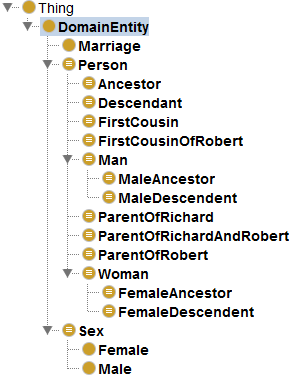
\includegraphics[width=.75\textwidth]{figures/class_hierarchy}
%\comment{WRONG TEXT, this is a Snapshot of an ADVANCED version of the class hierarchy!}
%\caption{An OWLviz picture of the \fhkb TBox as it now stands}
%\label{fig:stage1}
%\end{figure}

\section{Describing Parentage in the \fhkb}
 
To finish off the foundations of the \fhkb we need to describe a person object's parentage. We know that each and every person has one mother and each and every person has one father. Here we are talking about biological mothers and fathers. The complexities of adoption and step parents are outside the  scope of this \fhkb tutorial.

\steps{Describing Parentage}{
\item Add the domain \person and the range \woman to the property \con{hasMother}. 
\item Do the same for the property \con{hasFather}, but give it the range \man;
\item Give the property \con{hasParent} domain and range of \person;
\item Run the reasoner.
}
\noindent The (inferred) property hierarchy in the \fhkb should look like that shown in Figure~\ref{fig:phparentage}. Notice that we have asserted the sub-property axioms on one side of the property hierarchy. Having done so, the reasoner uses those axioms, together with the inverses, to work out the property hierarchy for the `other side'.

We make \con{hasMother} functional, as any one person object can hold only one \con{hasMother} property to a distinct \woman object. The range of \con{hasMother} is \woman, as a mother has to be a woman. The \person object holding the \con{hasMother} property can be either a man or a woman, so we have the domain constraint as \person; this means any object holding a \con{hasMother} property will be inferred to be a \person. Similarly, any object at the right-hand end of a \con{hasMother} property will be inferred to be a \woman, which is the result we need. The same reasoning goes for \con{hasFather} and \con{hasParent}, with the sex constraints on the latter being only \person. The inverses of the two functional sub-properties of \con{hasParent} are not themselves functional. After all, a \woman can be the mother of many \person objects, but each \person object can   have only one mother.

\begin{figure}
\begin{center}
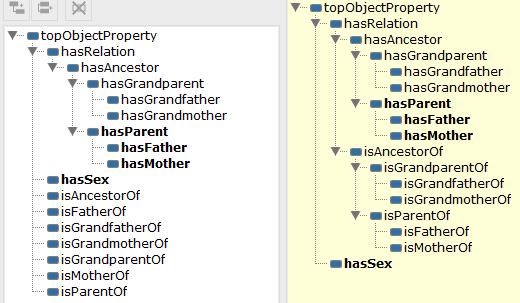
\includegraphics[width=\figwidth]{figures/new/prophierparentage}
\caption{The property hierarchy with the \con{hasSex} and the parentage properties}\label{fig:phparentage}
\end{center}
\end{figure}

\steps{Restrict \person class}{
\item As each and every person has a mother and each and every person has a father, place restrictions on the \person class as shown below.
}

\owlcode{
Class: Person
    
    SubClassOf: 
        DomainEntity,
         (hasFather some Man),
         (hasMother some Woman),
         (hasSex some Sex)
    
    DisjointWith: 
        Sex
}

\begin{figure}
\begin{center}
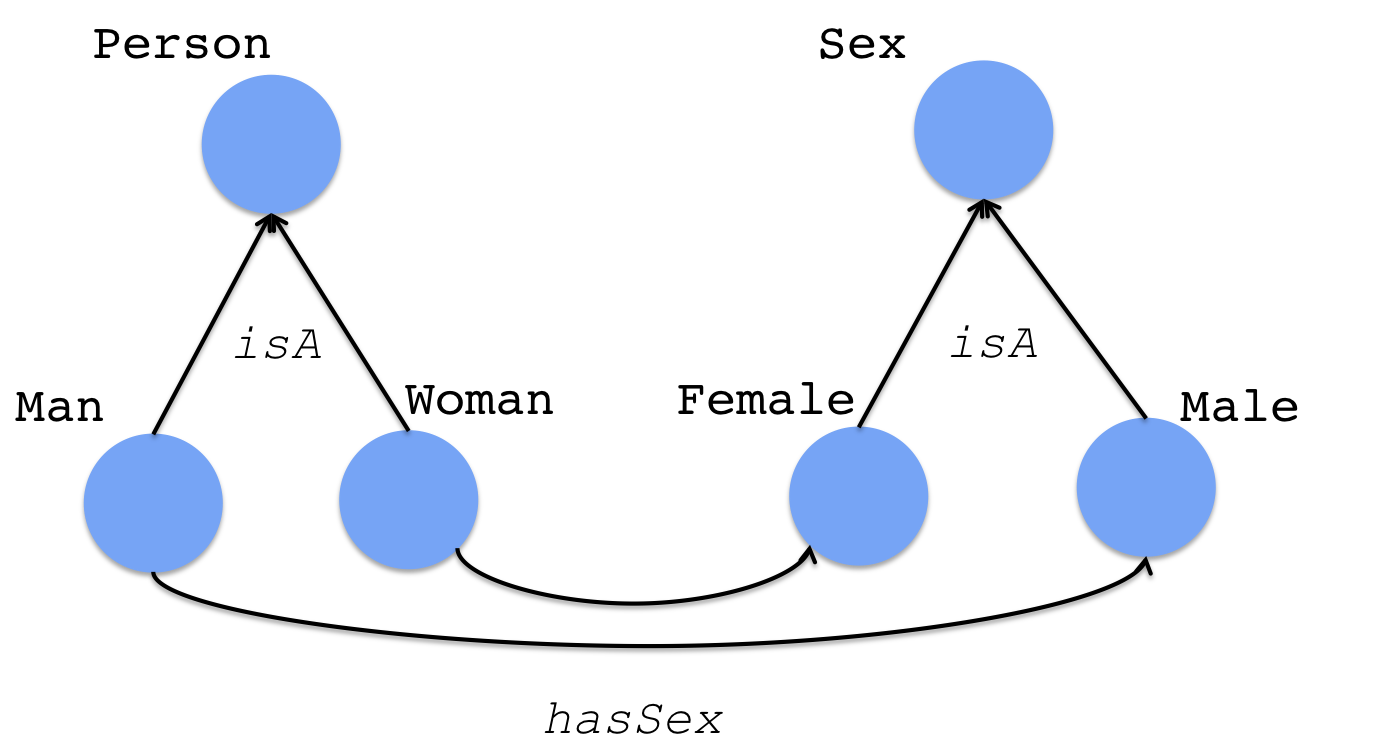
\includegraphics[width=\figwidth]{figures/sex}\caption{the core TBox for the \fhkb with the \person and \con{Sex} classes.}\label{fig:person_sex}
\end{center}
\end{figure}

\steps{DL queries for people and sex}{
\item Issue the DL queries for \person, \man and \woman; look at the answers and count the numbers in each class; which individuals have no sex and why?
\item You should find that many people have been inferred to be either \man or \woman, but some are, as we will see below, only inferred to be \person.
}

The domain and range constraints on our properties have also driven some entailments. We have not asserted that \ids is a member of \man, but the range constraint on \con{hasFather} (or the inferred domain constraint on the \con{isFatherOf} relation) has enabled this inference to be made. This goes for any individual that is the right-hand-side (either inferred or asserted) of either \con{hasFather} or \con{hasMother} (where the range is that of \woman). For \rds, however, he is only the left-hand-side of an \con{hasFather} or an \con{hasMother} property, so we've only entailed that this individual is a member of \person.

% 

%\section{Asserting an Individual's Type}
%Individuals are members of classes. We can either state to which class an individual belongs, infer to which class it belongs because of what we have said about that or another individual, or we can rely on both. Sometimes, of course, we can say or infer things about an individual that means our ontology becomes inconsistent (and we will make this happen at some point).
%
%First we need some individuals, so do the following in a new file for the individuals in the \fhkb:
%\steps{Create individuals}{
%\item Create a new ontology called \texttt{fhkb-a.owl};
%\item Create the following individuals: 
%\begin{itemize}
%\item Robert David Bright (1965;
%\item David Bright (1934;
%\item Richard John Bright (1962;
%\item Margaret Grace Rever (1934;
%\end{itemize} 
%For each individual, create a IRI fragment with the given names followed by family name, followed by birth year, each separated by underscores. 
%
%
%%Save these `bare' individuals in files \texttt{fhkb-a1} and \texttt{fhkb-a2}.
%\item For each of the individuals in file \texttt{fhkb-a1}, assert the type of each individual to be either \man or \woman, as described in the OWL below.
%\item In the file \texttt{fhkb-a2}, assert sex types about each person individual using the \con{hasSex} property. An example of such an assertion can be seen below. 
%}
%
%\owlcode{
%Individual: grant\_plinth
%	
%	Annotations:
%		label "Grant Plinth"
%
%	types:
%		Man
%
%Individual: grant\_plinth
%	
%	Annotations:
%		label "Grant Plinth"
%
%	types:
%		hasSex some Maleness
%}
%
%These are ways of asserting the \textbf{type} of an individual. In the first example above we just give the type of the individual `Grant Plinth' as Man -- the class we defined in Chapter~\ref{chap:person} as `A person with sex male'. In the second example, we are not using the \man class as a type, but we are essentially doing the same thing. By giving the type of `Grant Plinth' as \con{hasSex some Maleness}, we are making him a member of the anonymous class of those entities \con{hasSex some Sex}. We can write class expressions of an arbitrary complexity in the type of an individual. Note that the domain of \con{hasSex} is \person, so we will infer any individual holding one of those \con{hasSex} properties  to be a member of the \person class. So, these two ways of asserting sex are really just the same. Note also that  we are not naming individual sex instances, we are just relating this individual to some anonymous sex instance. As \con{hasSex} is functional, this individual is related to only one distinct sex instance.
%
%We can now use each of these ways of modelling sex of individuals to show off some inferences made by the reasoners.
%
%\steps{Run the reasoner}{
%\item Run the reasoner on file \texttt{fhkb-a1}.
%\item Issue a DL query of \man and then \woman (make sure that you are checking the correct boxes in the DL Query tab if you are using \protege);
%\item Ask the DL query \con{hasSex some Maleness} and see what results are returned.
%\item Ask the DL query \con{hasFather some Man} and see what results are returned.
%\item Load in the file \texttt{fhkb-a2} and repeat the procedure, recording your results.
%}
%
%For both the \texttt{fhkb-a1} and the \texttt{fhkb-a2}, the following results should have been seen:
%\begin{itemize}
%\item For \man or \con{hasSex some Maleness}: 
%\begin{itemize}
%\item \con{Robert\_David\_Bright\_1965}
%\item \con{David\_Bright\_1934}
%\item \con{Richard\_John\_Bright\_1962}
%\end{itemize} 
%\item For \woman or \con{hasSex some Femaleness}: \con{Margaret\_Grace\_Rever\_1934}
%\item For \con{hasFather some Man} all four family members are returned.
%\end{itemize}
\section{Who has a father?}

In our description of the \person class we have said that each and every instance of the class \person has a father (the same goes for mothers). So, when we ask the query `which individuals have a father', we get all the instances of \person back, even though we have said nothing about the specific parentage of each \person. We do not know who their mothers and fathers are, but we know that they have one of each. We know all the individuals so far entered are members of the \person class;  when  asserting the type to be either \man or \woman (each of which is a subclass of \person), we infer that each is a person. When asserting the type of each individual via the \con{hasSex} property, we know each is a \person, as the domain of \con{hasSex} is the \person class. As we have also given the right-hand side of \con{hasSex} as either \male  or \female, we have given sufficient information to recognise each of these \person instances to be members of either \man or \woman.

\section{Filling in Domains and Ranges for the \fhkb Properties}

So far we have not systematically added domains and ranges to the properties in the \fhkb. As a reminder, when a property has a domain of \con{X} any object holding that property will be inferred to be a member of class \con{X}. A domain doesn't add a constraint that only members of class \con{X} hold that property; it is a strong implication of class membership. Similarly, a property holding a range implies that an object acting as right-hand-side to a property will be inferred to be of that class. We have already seen above that we can use domains and ranges to imply the sex of people within the \fhkb.

Do the following:
\steps{Domains and Ranges}{
\item Make sure the appropriate \person, \man and \woman are domains and ranges for \con{hasFather}, \con{hasMother} and \con{hasParent}.
\item Run the reasoner and look at the property hierarchy.
\item Also look at the properties \con{hasAncestor}, \con{hasGrandparent},  \con{hasUncle} and so on; look to see what domains and ranges are found. Add any domains and ranges explicitly as necessary.
}

\warning{\protege for example in its current version (November 2015) does not visualise inherited domains and ranges in the same way as it shows inferred inverse relations.}

We typically assert more domains and ranges than strictly necessary. For example, if we say that \con{hasParent} has the domain \person, this means that every object \con{x} that is connected to another object \con{y} via the \con{hasParent} relation must be a \person. Let us assume the only thing we said about \con{x} and \con{y} is that they are connected by a \con{hasMother} relation. Since this implies that \con{x} and \con{y} are also connected by a \con{hasParent} relation (\con{hasMother} is a sub-property of \con{hasParent}) we do \emph{not} have to assert that \con{hasFather} has the domain of \person; it is implied by what we know about the domain and range of \con{hasParent}. 

In order to remove as many assertions as possible, we may therefore choose to assert as much as we know starting from the top of the hierarchy, and only ever adding a domain if we want to constrain the already inferred domain even further (or range respectively). For example, in our case, we could have chosen to assert \person to be the domain of \con{hasRelation}. Since \con{hasRelation} is symmetric, it will also infer \person to be the range. We do not need to say anything for \con{hasAncestor} or \con{hasParent}, and only if we want to constrain the domain or range further (like in the case of \con{hasFather} by making the range \con{Man}) do we need to actually assert something. It is worth noting that because we have built the object property hierarchy from the bottom (\con{hasMother} etc.) we have ended up asserting more than necessary.

\section{Inconsistencies}

From the Pizza Tutorial and other work with OWL you should have seen some \emph{unsatisfiabilities}. In \protege this is highlighted by classes going `red' and being subclasses of \con{Nothing}; that is, they can have no instances in that model.

\steps{Inconsistencies}{
\item Add the fact \irds \con{hasMother} \ids.
\item Run the classifier and see what happens.
\item Remove that fact and run the classifier again.
\item Now add the fact that \irds \con{hasMother} \iiea{}. 
\item Run the classifier and see what happens.
\item Add and remove the functional characteristic to these properties and see what happens.
}

After asserting the first fact it should be reported by the reasoner that the ontology is \emph{inconsistent}. 
This means, in lay terms, that the model you've provided in the ontology cannot accommodate the facts you've provided in the fact assertions  in your ABox---that is, there is an inconsistency between the facts and the ontology\ldots
The ontology is inconsistent because \ids is being inferred to be a \man and a \woman at the same time which is inconsistent with what we have said in the \fhkb. 
%\comment{put the justification in here and check if that is available in \protege.}

When we, however, say that \rds has two different mothers, nothing bad happens! Our domain knowledge says that the two women are different, but the reasoner does not know this as yet\ldots; Iris Ellen Archer  and Margaret Grace Rever may be the same person; we have to tell the reasoner that they are different. For the same reason the functional characteristic also has no effect until the reasoner `knows' that the individuals are different. \herebedragons We will do this in Section~\ref{sec:countchildren} and live with this	 `fault' for the moment.

%\begin{tasks}
%\item Make all the individuals different by adding a `different individuals' axiom; \comment{Add a comment; remove that axiom and reintroduce it in \ref%{sec:countchildren}}
%\item Run the reasoner and look at the results;
%\item Remove the offending axiom about \rds having Iris Elenn Archer as a mother, re-run the classifier and check the results.
%\end{tasks}
%\taskcont

\section{Adding Some Defined Classes for Ancestors and so on}
\label{sec:ancest-defined}

\steps{Adding defined classes}{
\item Add a defined class for \con{Ancestor}, \con{MaleAncestor}, \con{FemaleAncestor};
\item Add a defined class for \con{Descendant}, \con{MaleDescendant} and \con{FemaleDescendant};
\item Run the reasoner and view  the resulting hierarchy.
}
The code for the classes looks like:
\\\\
\owlcode{
Class: Ancestor
	EquivalentTo: Person
		and isAncestorOf some Person

Class: FemaleAncestor
	EquivalentTo: Woman
	and isAncestorOf some Person

Class: Descendant
	EquivalentTo: Person
		and hasAncestor some Person

Class: MaleDescendant
	EquivalentTo: Man
		and hasAncestor some Person
} 
\\\\
The TBox after reasoning can be seen in Figure~\ref{fig:equiv}. Notice that the reasoner has inferred that several of the classes are equivalent or `the same'. These are: Descendant and Person; MaleDescendant and Man, FemaleDescendant and Woman.
%\begin{itemize}
%\item Ancestor and Parent; Father and Male Ancestor; [NO! There is no Parent and Father class]
%\item 
%\end{itemize}

The reasoner has used the axioms within the ontology to infer that all the instances of \con{Person} are also instances of the class \con{Descendant} and that all the instances of \con{Woman} are also the same instances as the class \con{Female Descendant}. This is intuitively true; all people are descendants -- they all have parents that have parents etc. and thus everyone is a descendant. All women are female people that have parents etc. As usual we should think about the objects within the classes and what we know about them. This time it is useful to think about the statements we have made about \person in this Chapter -- that all instances of \person have a father and a mother; add to this the information from the property hierarchy and we know that all instances of \person have parents and ancestors. We have repeated all of this in our new defined classes for \con{Ancestor} and \con{Descendant} and the reasoner has highlighted this information.

\begin{figure}
\begin{center}
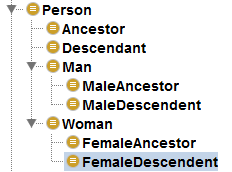
\includegraphics[width=\figwidth]{figures/new/descendent_ancestor_defined_classes.PNG}\caption{The defined classes from Section~\ref{sec:ancest-defined} in the \fhkb's growing class hierarchy}\label{fig:equiv}
\end{center}
\end{figure}

\steps{More Ancestors}{
\item Query for \con{MaleDescendant}. You should get \con{Man} back - they are equivalent (and this makes sense).
\item As an additional exercise, also add in properties for forefathers and foremothers. You will follow the same pattern as for \con{hasAncestor}, but adding in, for instance, \con{hasFather} as the sub-property of the transitive super-property of \con{hasForefather} and setting the domains and ranges appropriately (or working out if they'll be inferred appropriately). Here we interpret a forefather as one's father's father etc. This isn't quite right, as a forefather is any male ancestor, but we'll do it that way anyway. You might want to play around with DL queries. Because of the blowup in inferred relationships, we decided to not include this pattern in the tutorial version of the \fhkb. 
}

\section{Summary}

Most of what we have done in this chapter is straight-forward OWL, all of which would have been met in the pizza tutorial. It is, however, a useful revision and it sets the stage for refining the \fhkb. Figure~\ref{fig:person_sex} shows the basic set-up we have in the \fhkb in terms of classes; we have a class to represent person, man and woman, all set-up with a description of sex, maleness and femaleness.  It is important to note, however, the approach we have taken: We have always thought in terms of the objects we are modelling. 

Here are some things that should now be understood upon completing this chapter:
\begin{enumerate}
\item Restrictions on a class in our TBox mean we know stuff about individuals that are members of that class, even though we have asserted no facts on those individuals. We have said, for instance, that all members of the class \person have a mother, so any individual asserted to be a \person must have a mother. We do not necessarily know who they are, but we know they have one.
\item Some precision is missing -- we only know \rds is a \person, not that he is a \man. This is because, so far, he only has the domain constraint of \con{hasMother} and \con{hasFather} to help out.
\item We can cause the ontology to be inconsistent, for example by providing facts that cannot be accommodated by the model of our ontology. In the example, \ds was inferred to be a member of two disjoint classes.
\end{enumerate}

Finally, we looked at some defined classes. We inferred equivalence between some classes where the extents of the classes were inferred to be the same -- in this case the extents of \con{Person} and \con{Descendant} are the same. That is, all the objects that can appear in \con{Person} will also be members of \con{Descendant}. We can check this implication intuitively -- all people are descendants of someone. Perhaps not the most profound inference of all time, but we did no real work to place this observation in the \fhkb.

\note{This last point is a good general observation. We can make the reasoner do work for us. The less maintenance we have to do in the \fhkb the better. This will be a principle that works throughout the tutorial.} 

\expressivity{SRIF}

\ctime{884}{256}{13}
\chapter{Exercise \arabic{excounter}}
\addtocounter{excounter}{1}
\herebedragons
\steps{Finding siblings}{
\item Add an object property \con{hasSibling} at the appropriate place to the object property hierarchy.
\item Decide whether it is symmetric  and/or transitive.
\item Add the property chain that will find siblings.
\item Run the reasoner.
\item Ask the DL query \con{hasSibling value \irds}; what's the problem?
\item Make \con{hasSibling} irreflexive, this should make it impossible for \rds to be his own brother. What happens? ask for an explanation (from a human being).
\item Add two sub-properties for \con{hasSibling}: \con{hasBrother} and \con{hasSister}. Decide on the transitivity, symmetry etc. for these properties and add an inverse property if you think it appropriate.
\item What sub-property chains do we need to make \con{hasBrother} work? Remember that we do not, as yet, know the sex of \rds and several other individuals.
\item The \con{isFatherOf} property has a range of \person; this will not determine the sex of a father's child. To fix this, make a property hierarchy of \con{hasChild}, \con{hasSon} and \con{hasDaughter}; add the appropriate domains and ranges.
\item Use an \con{EquivalentProperty} axiom to tie \con{hasChild} to an appropriate existing object property.
\item Add \con{hasSon} and \con{hasDaughter} assertions to the individuals.
\item Add sub-property chains to \con{hasBrother} and \con{hasSister} using these new properties; run the reasoner and test the answers with DL queries.
\item Inspect the object hierarchy.
}
\chapter{Individuals in Class Expressions}
\label{chap:nominal}

In this chapter you will:
\begin{enumerate}
\item Use individuals within class expressions;
\item Make classes to find Robert and Richard's parents, ancestors, and so on;
\item Explore equivalence of such classes;
\item Re-visit the closed world.
\end{enumerate}

\snapshot{There is a snapshot of the ontology as required at this point in the tutorial available at \fhkbhome.}

\section{Richard and Robert's Parents and Ancestors}

So far we have only used object properties between unspecified objects. We can, however, specify a specific individual to act at the right-hand-side of a class restriction or type assertion on an individual. The basic syntax for so-called \emph{nominals} is:
\\\\
\owlcode{
Class: ParentOfRobert

	EquivalentTo: Person
		and isParentOf value \irds
}
\\\\
This is an equivalence axiom that recognises any \indiv that is a \person and a parent of \rds.

\steps{Robert and Richards parents}{
\item Create the class \con{ParentOfRobert} as described above;
\item Classify -- inspect where the class is placed in the \fhkb TBox and look at which individuals classify as members of the class;
\item Do the same for a class with the value of \irjs and classify;
\item Finally create a class ParentOfRichardAndRobert, defining it as \con{Person and isParentOf some \{{\irds},{\irjs}\}}; again see what happens on classification. Note that the expressions \texttt{isMotherOf value \irds} and \texttt{isMotherOf some \{\irds\}} are practically identical. The only difference is that using \texttt{value}, you can only specify one individual, while \texttt{some} relates to a class (a set of individuals).
}

We see that these queries work and that we can create more complex nominal based class expressions. The disjunction above is
\\\\
\owlcode{
isParentOf some \{Robert\_David\_Bright\_1965, Richard\_John\_Bright\_1965\}
}
\\\\
The `\{' and `\}' are a bit of syntax that says `here's a class of individual'.

We also see that the classes for the parents of \rds and \rjs have the same members according to the \fhkb, but that the two classes are not inferred to be equivalent. Our domain knowledge indicates the two classes have the same extents (members) and thus the classes are equivalent, but the automated reasoner does not make this inference. As usual, this is because the \fhkb has not given the automated reasoner enough information to make such an inference.

\section{Closing Down What we Know About Parents and Siblings}
\label{sec:nom_owa}

The classes describing the parents of Richard and Robert are not equivalent, even though, as humans, we know their classes of parent are the same. We need more constraints so that it is known that the four parents are the only ones that exist. We can try this by closing down what we know about the immediate family of \rds.

In Chapter~\ref{chap:person} we described that a \person has exactly one \woman and exactly one \man as mother and father (by saying that the \con{hasMother} and \con{hasFather} properties are functional and thus only one of each may be held by any one individual to distinct individuals). The parent properties are defined in terms of \con{hasParent}, \con{hasMother} and \con{hasFather}. The latter two imply \con{hasParent}. The two sub-properties are functional, but there are no constraints on \con{hasParent}, so an individual can hold many instances of this property. So, there is no information in the \fhkb to say a \person has only two parents (we say there is one mother and one father, but not that there are only two parents). Thus Robert and Richard could have other parents and other grandparents than those in the \fhkb; we have to close down our descriptions so that only two parents are possible. There are two ways of doing this:
\begin{enumerate}
\item Using qualified cardinality constraints in a class restriction;
\item Putting a covering axiom on \con{hasParent} in the same way as we did for \con{Sex} in Chapter~\ref{chap:person}.
\end{enumerate}

\steps{Closing the \person class}{
\item Add the restriction \con{hasParent exactly 2 Person} to the class \person;
\item Run the reasoner;
\item Inspect the hierarchy to see where \con{ParentOfRobert} and \con{ParentOfRichard} are placed and whether or not they are found to be equivalent; 
\item Now add the restriction \con{hasParent max 2 Person} to the class \person;
\item Run the reasoner (taking note of how long the reasoning takes) and take another look.

}

We find that these two classes are equivalent; we have supplied enough information to infer that these two classes are equivalent. So, we know that option one above works, but what about option two? \herebedragons
This takes a bit of care to think through, but the  basic thing is to think about how many ways there are to have a \con{hasParent} relationship between two individuals. We know that we can have either a \con{hasFather} or a \con{hasMother} property between two individuals; we also know that we can have only one of each of these properties between an individual and a distinct individual. However, the open world assumption tells us that there may be other ways of having a \con{hasParent} property between two individuals; we've not closed the possibilities. By putting on the \con{hasParent exactly 2 Person} restriction on the \person class, we are effectively closing down the options for ways that a person can have parents; we know because of the functional characteristic on \con{hasMother} and \con{hasFather} that we can have only one of each of these and the two restrictions say that one of each must exist. So, we know we have two ways of having a parent on each \person individual. So, when we say that there are exactly two parents (no more and no less) we have closed down the world of having parents---thus these two classes can be inferred  to be equivalent. It is also worth noting that this extra axiom on the \person class will make the reasoner run much more slowly.

Finally, for option~2, we have no way of placing a covering axiom on a property. What we'd like to be able to state is something like:
\\\\
\owlcode{
ObjectProperty: hasParent

	EquivalentTo: hasFather or hasMother
}
\\
\noindent but we can't.

\section{Summary}
For practice, do the following:
\steps{Additional Practice}{
\item Add lots more classes using members of the ABox as nominals;
\item Make complex expressions using nominals;
\item After each addition of a nominal, classify and see what has been inferred within the \fhkb.
\item See if you can make classes for \con{GrandparentOfRobert} and \con{GrandparentOfRichard} and make them inferred to be equivalent.
}

In this chapter we have seen the use of individuals within class expressions. It allows us to make useful queries and class definitions. The main things to note is that it can be done and that there is some syntax involved. More importantly, some inferences may not be as expected due to the open world assumption in OWL.

\dragon{By now you might have noticed a significant increase in the time the reasoner needs to classify.
Closing down what we know about family relationships takes its toll on the reasoner performance, especially the usage of \con{hasParent exactly 2 Person}. At this point we recommend rewriting this axiom to \con{hasParent max 2 Person}. It gives us most of what we need, but has a little less negative impact on the reasoning time.}
\\

\expressivity{SROIQ}

\ctime{2067273}{529}{147}
\chapter{Data Properties in the \fhkb}
\label{chap:data}
 
We now have some individuals with some basic object properties between individuals. \owlii, however, also has data properties that can relate an object or individual to some item of data. There are data about a \person, such as years of events and names etc. So, in this Chapter you will:
\begin{enumerate}
\item Make some data properties to describe event years to people;
\item Create some simple defined classes that group people by when they were born;
\item Try counting the numbers of children people have\ldots
\item Deal with the open world assumption;
\item Add given and family names to individuals in the \fhkb.
\end{enumerate}

\snapshot{There is a snapshot of the ontology as required at this point in the tutorial available at \fhkbhome.}

\section{Adding Some Data Properties for Event Years}

Everyone has a birth year; death year; and some have a marriage year and so on. We can model these simply with data properties and an integer as a filler. \owlii has a DateTime datatype, where it is possible to specify a precise time and date down to a second.\footnote{\url{http://www.w3.org/TR/2008/WD-owl2-quick-reference-20081202/#Built-in_Datatypes_and_Facets}} This proves cumbersome (see \url{http://robertdavidstevens.wordpress.com/2011/05/05/using-the-datetime-data-type-to-describe-birthdays/} for details); all we need is a simple indication of the year in which a person was born. Of course, the integer type has a zero, which the Gregorian calendar for which we use integer as a proxy does not, but integer is sufficient to our needs. Also, there are various ontological treatments  of time and information about people (this extends to names etc. as well), but we gloss over that here---that's another tutorial.

We can have dates for birth, death and (eventually) marriage (see Chapter~\ref{chap:marriage}) and we can just think of these as event years. We can make a little hierarchy of event years as shown in Figure~\ref{fig:data_hierarchy}).

\steps{Create a data property hierarchy}{
\item Create the data property \con{hasEventYear} with range integer and domain \person;
\item Create the data property \con{hasBirthYear} and make it a sub-property of \con{hasEventYear} (that way, the domain and range of \con{hasEventYear} are inherited);
\item Create the data property \con{hasDeathYear} and make it a sub-property of \con{hasEventYear};
\item For each individual add the birth years shown in Table~\ref{tab:familydata} (see appendix). You do not actually have to go back to the table---it is easier to read the birth years simply off the individual names.
}
\snapshot{Again, asserting birth years for all individuals can be a bit tedious. The reader can find a convenience snapshot of the ontology at this stage at \fhkbhome.
}

We now have an ABox with individuals with fact assertions to data indicating a birth year. We can, if we wish, also add a class restriction to the \person class saying that each and every instance of the class \person holds a data property to an integer and that this property is called `hasBirthYear'. As usual when deciding whether to place such a restriction upon a class, ask whether it is true that each and every instance of the class holds that property; this is exactly the same as we did for the object properties in Chapter~\ref{chap:person}. Everyone does have a birth year, even if it is not known.

Once birth years have been added to our individuals, we can start asking some questions. 

\steps{DL queries}{
\item Use a DL query to ask: \begin{itemize}
\item \person born after 1960;
\item \person born in the 1960s;
\item \person born in the 1800s;
\item \person that has fewer than three children;
\item \person that has more than three children.
\end{itemize}
}

The DL query for people born in the 1960s is:
\\\\
\owlcode{
Person and hasBirthYear some int[>= 1960, < 1970]
}

This kind of interval is known as a facet.

\subsection{Counting Numbers of Children}
\label{sec:countchildren}

The last two queries in the list do not work as expected. We have asked, for instance, for \person that have more than three children, but we get no members of \person in the answer, though we know that there are some in the \fhkb (e.g., \ijb). This is because there is not enough information in the \fhkb to tell that this person has more than three \textbf{different} people as children. As humans we can look at the four children of John Bright and know that they are different -- for instance, they all have different birth years. The automated reasoner, however, does not know that a \person can only have one birth year.

\steps{Make a functional object property}{
\item Make the property \con{hasBirthYear} functional. 
\item Ask the query for \person that has more than three children again.
}

This time the query should work. All the other event year properties should be made functional, expect \con{hasEventYear}, as one individual can have many event years. As the children have different birth years and an individual can only hold one \con{hasBirthYear} property, then these people must be distinct entities.

Of course, making birth year functional is not a reliable way of ensuring that the automated reasoner knows that the individual are different. It is possible for two \person to have the same birth year within the same family -- twins and so on. \ipwb has three children, two of which are twins, so will not be a member of the class of people with at least three children. So, we use the \textbf{different individuals} axiom. Most tools, including \protege, have a feature that allows all individuals to be made different.

\steps{Make all individuals different}{
\item Make all individuals different;
\item Ask the above queries again.
}

From now on, every time you add individuals, make sure the different individuals axiom is updated.

\section{The Open World Assumption}

We have met again the open world assumption and its importance in the \fhkb. In the use of the functional characteristic on the \con{hasBirthYear} property, we saw one way of constraining the interpretation of numbers of children. We also introduced the `different individuals' axiom as a way of making all individuals in a knowledge base distinct. There are more questions, however, for which we need more ways of closing down the openness of \owlii.

Take the questions:
\begin{itemize}
\item People that have exactly two children;
\item People that have only brothers;
\item People that have only female children.
\end{itemize}

We can only answer these questions if we locally close the world.\herebedragons  We have said that David and Margaret have two children, Richard and Robert, but we have not said that there are not any others. As usual, try not to apply your domain knowledge too much; ask yourself what the automated reasoner actually knows. As we have the open world assumption, the reasoner will assume, unless otherwise said, that there could be more children; it simply doesn't know.

Think of a railway journey enquiry system. If I ask a standard closed world system about the possible routes by rail, between Manchester and Buenos Aires, the answer will be 'none', as there are none described in the system. With the open world assumption, if there is no information in the system then the answer to the same question will simply be `I don't know'. We have to explicitly say that there is no railway route from Manchester to Buenos Aires for the right answer to come back.

We have to do the same thing in OWL. We have to say that David and Margaret have only two children. We do this with a \textbf{type assertion} on individuals . So far we have only used fact assertions. A type assertion to close down \ds' parentage looks like this:
\\\\
\owlcode{
isParentOf only \{\irds, \irjs\}
}

This has the same meaning as the closure axioms that you should be familiar with on classes. We are saying that the only fillers that can appear on the right-hand-side of the \con{isParentOf} property on this individual are the two individuals for Richard and Robert. We use the braces to represent the set of these two individuals.\herebedragons

\steps{Make a closure axiom}{
\item Add the closure assertion above to \ds;
\item Issue the DL query \con{isParentOf exactly 2 Person}.
}

The last query should return the answer of \ds. Closing down the whole \fhkb ABox is a chore and would really have to be done programmatically. OWL scripting languages such as the Ontology Preprocessing Language\footnote{\url{http://oppl2.sourceforge.net}} (OPPL)~\cite{oppl} can help here. Also going directly to the OWL API~\cite{owlapi}\footnote{\url{http://owlapi.sourceforge.net/}}, if you know what you are doing, is another route. 
\\\\
\dragon{Adding all these closure type assertions can slow down the reasoner; so think about the needs of your system -- just adding it `because it is right' is not necessarily the right route.}


%\comment{the K-operator}

%\rds has only one father, but \ds may have any old nubmer of children; how do we close it?

\section{Adding Given and Family Names}

We also want to add some other useful data facts to people -- their names. We have been putting names as part of labels on individuals, but data fact assertions make sense to separate out family and given names so that we can ask questions such as `give me all people with the family name Bright and the first given name of either James or William'. A person's name is a fact about that person and is more, in this case, than just a label of the representation of that person. So, we want family names and given names. A person may have more than one given name -- `Robert David', for instance -- and an arbitrary number of given names can be held. For the \fhkb, we have simply created two data properties of \con{hasFirstGivenName} and \con{hasSecondGivenName}). Ideally, it would be good to have some index on the property to given name position, but OWL has no n-ary relationships. Otherwise, we could reify the \con{hasGivenName} property into a class of objects, such as the following:
\\\\
\owlcode{
Class: GivenName

SubClassOf:hasValue some String,

	hasPosition some Integer
}
\\\\
\noindent but it is really rather too much trouble for the resulting query potential.

As already shown, we will use data properties relating instances of \person to strings. We want to distinguish family and given names, and then different positions of given names through simple conflating of position into the property name. Figure~\ref{fig:data_hierarchy} shows the intended data property hierarchy.

\begin{figure}
\begin{center}
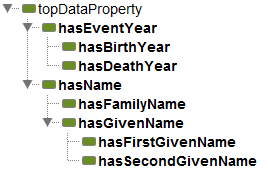
\includegraphics[width=\figwidth]{figures/new/event_name_hierarchy.PNG}\caption{The event year and name data property hierarchies in the \fhkb.}\label{fig:data_hierarchy}
\end{center}
\end{figure}

Do the following:
\steps{Data properties}{
\item Create the data properties as described in Figure~\ref{fig:data_hierarchy};
\item Give the \con{hasName} property the domain of \person and the range of \con{String};
\item Make the leaf properties of given names functional;
\item Add the names shown in Table~\ref{tab:familydata} (appendix); Again, it may be easier to read the names of the individual names.
\item Ask the questions:
\subitem all the people with the first given name `James';
\subitem all the people with the first given name `William';
\item All the people with the given name `William';
\item All the people with the given name `William' and the family name `Bright'.
}

The name data property hierarchy and the queries using those properties displays what now should be familiar.
Sub-properties that imply the super-property. So, when we ask \con{hasFirstGivenName value "William"} and then the query \con{hasGivenName value value "William"} we can expect different answers. There are people with `William' as either first or second given name and asking the question with the super-property for given names will collect both first and second given names.

\section{Summary}

We have used data properties that link objects to data such as string, integer, floats and Booleans etc. OWL uses the XML data types. We have seen a simple use of data properties to simulate birth years. The full \fhkb also uses them to place names (given and family) on individuals as strings. This means one can ask for the \person with the given name "James", of which there are many in the \fhkb.

Most importantly we have re-visited the open world assumption and its implications for querying an OWL ABox. We have looked at ways in which the ABox can be closed down -- unreliably via the functional characteristic (in this particular case) and more generally via type assertions.

All the DL queries used in this chapter can also serve as defined classes in the TBox. It is a useful exercise to progressively add more defined classes to the \fhkb TBox. Make more complex queries, make them into defined classes and inspect where they appear in the class hierarchy. 
\\
\expressivity{SROIQ(D)}

\ctime{1891157}{1134}{201}

\note{Note that we now cover the whole range of expressivity of OWL~2. HermiT at least is impossibly slow by now. This may be because HermiT does more work than the others. For now, we recommend to use either Pellet or FaCT++.}
\chapter{Cousins in the \fhkb}
\label{chap:cousins}
\taskstart 

In this Chapter you will
\begin{enumerate}
\item Revise or get to know about degrees and removes of cousin;
\item Add the properties and sub-property chains for first and second cousins;
\item Add properties and sub-property chains for some removes of cousins;
\item Find out that the siblings debacle haunts us still;
\item Add a defined class that does first cousins properly.
\end{enumerate}

\snapshot{There is a snapshot of the ontology as required at this point in the tutorial available at \fhkbhome.}

\dragon{Be warned; from here on the reasoner can start running slowly! Please see warning at the beginning of the last chapter for more information.}

\section{Introducing Cousins}
\label{sec:cousin_intro}

Cousins can be confusing, but here is a brief summary:
\begin{itemize}
\item First cousins share a grandparent, but are not siblings;
\item Second cousins share a great grandparent, but are not first cousins or siblings;
\item Degrees such as first and second cousin give the distance to the nearest common ancestor;
\item Removes give differences in generation. So, my Dad's first cousins (his generation) are my (\rds's) first cousins once removed.
\end{itemize}
Simply, my first cousins are my parent's sibling's children. As usual, we can think about the objects and put in place some sub-property chains.

\section{First Cousins}

Figure~\ref{fig:first_cousins} shows the sub-property chain for first cousins. As usual, think at the object level; to get to the first cousins of \rds, we go to the parents of \rds, to their siblings and then to their children. We go up, along and down. The OWL for this could be:

\owlcode{
ObjectProperty: hasFirstCousin

    SubPropertyOf: 
        hasCousin
    
    SubPropertyChain: 
        hasParent o hasSibling o hasChild
    
    Characteristics: 
        Symmetric
}

\begin{figure}
\begin{center}
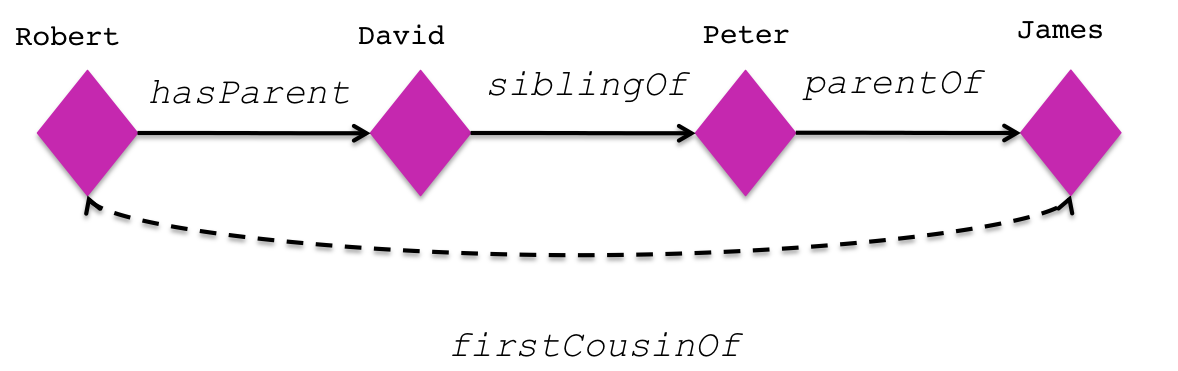
\includegraphics[width=\figwidth]{figures/cousin}
\caption{Tracing out the sub-property chain for cousins going from a child to a parent, to its sibling, and down to its child, a cousin}
\label{fig:first_cousins}
\end{center}
\end{figure}

Note that we follow the definitions in Section~\ref{sec:cousin_intro} of first cousins sharing a grandparent, but not a parent. The sub-property chain goes up to children of a grandparent (a given person's parents), along to siblings and down to their children. We do not want this property to be transitive. One's cousins are not necessarily my cousins. The blood uncles of \rds have children that are his cousins. These first cousins, however, also have a mother that is not a blood relation of \rds and the mother's sibling's children are not cousins of \rds.  

We do, however, want the property to be symmetric. One's cousins have one's-self as a cousin.

We need to place the cousin properties in the growing object property hierarchy. Cousins are obviously blood relations, but not ancestors, so they go off to one side, underneath \con{hasBloodrelation}. We should group the different removes and degree of cousin underneath one \con{hasCousin} property and this we will do.

Do the following:
\steps{First cousins}{
\item Add the property of \con{hasCousin} to the hierarchy underneath \con{hasBloodrelation};
\item Add \con{hasFirstCousin} underneath this property;
\item Add the sub-property chain as described above;
\item Run the reasoner and look at the first cousins of \rds.
}

You should see the following people as first cousins of \rds: Mark Anthony Heath, Nicholas Charles Heath, Mark Bright, Ian Bright, Janet Bright, William Bright, James Bright, Julie Bright, Clare Bright, Richard John Bright and Robert David Bright. The last two, as should be expected, are first cousins of \rds and this is not correct. As \ds will be his own brother, his children are his own nieces and nephews and thus the cousins of his own children. Our inability to infer siblings correctly in the \fhkb haunts us still and will continue to do so.

\dragon{Although the last query for the cousins of \rds should return the same results for every reasoner, we have had experiences where the results differ.}

\section{Other Degrees and Removes of Cousin}

Other degrees of cousins follow the same pattern as for first cousins; we go up, along and down. For second cousins we go up from a given individual to children of a great grandparent, along to their siblings and down to their grandchildren. The following object property declaration is for second cousins (note it uses the \con{isGrandparentOf} and its inverse properties, though the parent properties could be used) :

\owlcode{
ObjectProperty: hasSecondCousin

    SubPropertyOf: 
        hasCousin
    
    SubPropertyChain: 
        hasGrandParent o hasSibling o isGrandParentOf
    
    Characteristics: 
        Symmetric
}

`\emph{Removes}' simply add in another `leg' of either `up' or `down' either side of the `along'---that is, think of the actual individuals involved and draw a little picture of blobs and lines---then trace your finger up, along and down to work out the sub-property chain. The following object property declaration does it for first cousins once removed (note that this has been done by putting this extra `leg' on to the \con{hasFirstCousin} property; the symmetry of the property makes it work either way around so that a given person is the first cousin once removed of his/her first cousins once removed): 
\\\\
\owlcode{
ObjectProperty: hasFirstCousinOnceRemoved

    SubPropertyOf: 
        hasCousin
    
    SubPropertyChain: 
        hasFirstCousin o hasChild
    
    Characteristics: 
        Symmetric
}
\\\\
To exercise the cousin properties do the following:
\steps{Cousin properties}{
\item Add properties for second degree cousins;
\item Add removes for first and second degree cousins;
\item Run the reasoner and check what we know about \rds' other types of cousin.
}
You should see that we see some peculiar inferences about \rds' cousins -- not only are his brother and himself his own cousins, but so are his father, mother, uncles and so on. This makes sense if we look at the general sibling problem, but also it helps to just trace the paths around. If we go up from one of \rds' true first cousins to a grandparent and down one parent relationship, we follow the first cousin once removed path and get to one of \rds' parents or uncles. This is not to be expected and we need a tighter definition that goes beyond sub-property chains so that we can exclude some implications from the \fhkb.
%\todo{check and finish}

\section{Doing First Cousins Properly}

As far as inferring first cousin facts for \rds, we have failed. More precisely, we have recalled all \rds's cousins, but the precision is not what we would desire. What we can do is ask for \rds' cousins, but then remove the children of \rds' parents. The following DL query achieves this:

\owlcode{
Person that hasFirstCousin value \irds 

and (not (hasFather value \ids) or not (hasMother value \imgs)
}
\\
This works, but only for a named individual. We could make a defined class for this query; we could also make a defined class \con{FirstCousin}, but it is not of much utility. We would have to make sure that people whose parents are not known to have siblings with children are excluded. That is, people are not `first cousins' whose only first cousins are themselves and their siblings. The following class does this:

\owlcode{
Class: FirstCousin

EquivalentTo: Person
	that hasFirstCousin some Person
}

\steps{Roberts first cousins}{
\item Make a defined class \con{FirstCousin} as shown above;
\item Make a defined class \con{FirstCousinOfRobert};
\item Create a DL query that looks at \irds first cousins and takes away the children of \irds' parents as shown above.
}
This gives some practice with negation. One is making a class and then `taking' some of it away -- `these, but not those'.\herebedragons 
%\todo{perhaps a bit ore about negation?}

\section{Summary}

We have now expanded the \fhkb to include most blood relationships. We have also found that cousins are hard to capture just using object properties and sub-property chains. Our broken sibling inferences mean that we have too many cousins inferred at the instance level. We can get cousins right at the class level by using our inference based cousins, then excluding some using negation. Perhaps not neat, but it works.

We have reinforced that we can just add more and more relationships to individuals by just adding more properties to our \fhkb object property hierarchy and adding more sub-property chains that use the object properties we have built up upon parentage and sibling properties; this is as it should be.
\\

\expressivity{SROIQ(D)}

\ctime{0}{111395}{868}
\chapter{Exercise \arabic{excounter}}
\addtocounter{excounter}{1}

\steps{In-laws: Modelling partnerships}{
\item Add the class \con{Partnership} to the \fhkb as a sibling of \person and make it disjoint with its primitive siblings.
\item Create the object properties \con{hasParticipant}, \con{hasMaleParticipant} and \con{hasFemaleParticipant} in the obvious object hierarchy, along with their inverses. \con{Partnership} is their common domain and add the obvious ranges to these properties.
\item Add a restriction of \con{hasParticipant min 2 Person} to the \con{Marriage} class.
\item Create the object properties \con{hasSpouse}, \con{hasWife} and \con{hasHusband} and inverses where appropriate (or use property characteristics when they are not). Use sub-property chains to infer when two individuals are husband and wife. \ds and \mgs were married in 1958; create an individual for this marriage (you can add a \con{hasMarriageYear} data property if you wish). John Bright and Joyce Gosport were married in 1954. Add another individual for this marriage.
\item Run the reasoner and ask DL queries to test what you have done.
\item Create new object properties for in-laws-brother-in-law, sister-in-law (hint: these last two have possible sub-property chains)  and sibling-in-law. You can also now add properties to find uncles- and aunts-in-law.
\item Run the reasoner, and ask DL queries to confirm that it all works.
\item Add these  two property hierarchies to the main object property hierarchy, reason and look at it.
}
\chapter{Extending the TBox}
\label{chap:tbox}

In this chapter you will:
\begin{enumerate}
\item Just add lots of defined classes for all the aspects we have covered in this \fhkb tutorial;
\item You will learn that the properties used in these defined classes must be chosen with care.
\end{enumerate}

\snapshot{There is a snapshot of the ontology as required at this point in the tutorial available at \fhkbhome.}

\section{Adding Defined Classes}

%\todo{Normalize class names in the following, whitespace, capitalisation}
Add the following defined classes:
\steps{Adding defined classes}{
\item Relation and blood relation;
\item Forefather and Foremother;
\item Grandparent, Grandfather and Grandmother;
\item GreatGrandparent, GreatGrandfather and GreatGrandmother;
\item GreatGrandparentOfRobert, GreatGrandfatherOfRobert and  GreatGrandMotherOfRobert
\item Daughter, Son, Brother, Sister, Child;
\item Aunt, Uncle, AuntInLaw, UncleInLaw, GreatAunt and GreatUncle; %removed great aunt great uncle
\item FirstCousin and SecondCousin;
\item First cousin once removed;
\item InLaw, MotherInLaw, FatherInLaw, ParentInLaw, SiblingInLaw, SisterInLaw, BrotherInLaw;
\item Any defined class for any property in the hierarchy and any nominal variant of these classes.
}

The three classes of \con{Child}, \con{Son} and \con{Daughter} are of note. They are coded in the following way:

\owlcode{
Class: Child
	EquivalentTo: Person
		that hasParent Some Person

Class: Son
	EquivalentTo: Man
		that hasParent Some Person

Class: Daughter
	EquivalentTo: Woman
		that hasParent Some Person
}

After running the reasoner, you will find that \con{Person} is found to be equivalent to \con{Child}; \con{Daughter} is equivalent to \con{Woman} and that \con{Son} is equivalent to \con{Man}. This does, of course, make sense -- each and every person is someone's child, each and every woman is someone's daughter. We will forget evolutionary time-scales where this might be thought to break down at some point -- all \con{Person} individuals are also \con{Descendant} individuals, but do we expect some molecule in some prebiotic soup to be a member of this class?

Nevertheless, within the scope of the \fhkb, such inferred equivalences are not unreasonable. They are also instructive; it is possible to have different intentional descriptions of a class and for them to have the same logical extents. You can see another example of this happening in the amino acids ontology, but for different reasons.

Taking \con{Grandparent} as an example class, there are two ways of writing the defined class:

\owlcode{
Class: Grandparent
	EquivalentTo: Person
		and isGrandparentOf some Person

Class: Grandparent
	EquivalentTo: Person
	and (isParentOf some (Person and (isParentOf some Person))
}

Each comes out at a different place in the class hierarchy. They both capture the right individuals as members (that is, those individuals in the ABox that are holding a \con{isGrandparentOf} property), but the class hierarchy is not correct. By definition, all grandparents are also parents, but the way the object property hierarchy works means that the first way of writing the defined class (with the \con{isGrandparentOf} property) is not subsumed by the class \con{Parent}. We want this to happen in any sensible class hierarchy, so we have to use the second pattern for all the classes, spelling out the sub-property path that implies the property such as \con{isGrandparentOf} within the equivalence axiom.

The reason for this need for the `long-form' is that the \con{isGrandparentOf} does not imply the \con{isParentOf} property. As described in Chapter~\ref{chap:ancestor} if this implication were the case, being a grandparent of \rds, for instance, would also imply that the same \person were a parent of \rds; an implication we do not want. As these two properties (\con{isParentOf} and \con{isGrandparentOf}) do not subsume each other means that the defined classes written according to pattern one above will not subsume each other in the class hierarchy. Thus we use the second pattern.
If we look at the class for grandparents of Robert:

\owlcode{
Class: GrandparentOfRobert

EquivalentTo: Person
		that isParentOf some (Person
			that isParentOf value \rds)
}

If we make the equivalent class for \rjs, apply the reasoner and look at the hierarchy, we see that the two classes are not logically equivalent, even though they have the same extents of William George Bright, Iris Ellen Archer, Charles Herbert Rever and Violet Sylvia Steward. We looked at this example in Section~\ref{sec:nom_owa}, where there is an explanation and solutions.

\begin{figure}
\begin{center}
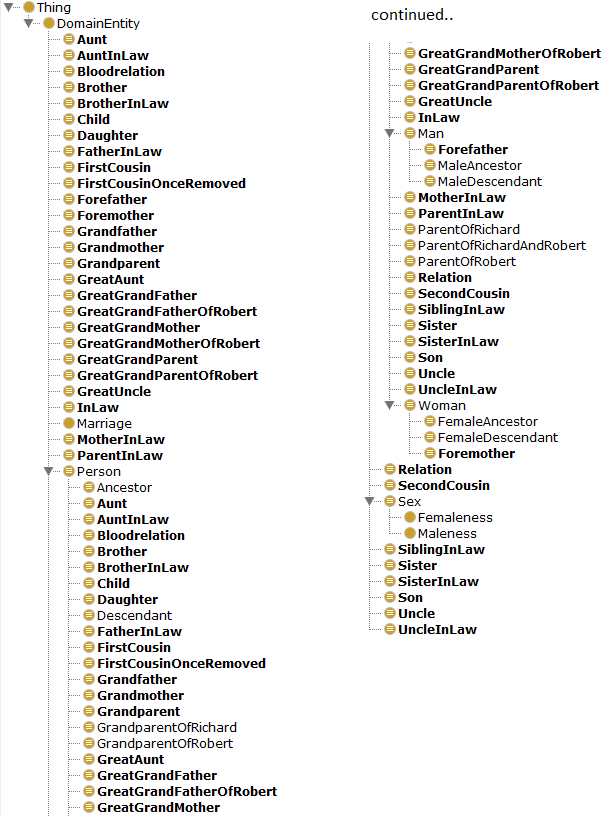
\includegraphics[width=\largefigwidth]{figures/class_hierachy_final_1}\caption{The full TBox hierarchy of the \fhkb}
\label{fig:tbox2}
\end{center}
\end{figure}

\section{Summary}

We can add defined classes based on each property we have put into the object property hierarchy. We see the expected hierarchy; as can be seen from Figure~\ref{fig:tbox2} it has an obvious symmetry based on sex. We also see a lot of equivalences inferred -- all women are daughters, as well as women descendants. Perhaps not the greatest insight ever gained, but it at least makes sense; all women must be daughters. It is instructive to use the explanation feature in \protege to look at why the reasoner has made these inferences. For example, take a look at the class \con{hasGrandmother some Woman} -- it is instructive to see how many there are.

Like the Chapter on marriage and in-law (Chapter~\ref{chap:marriage}), this chapter has largely been revision. One thing of note is, however, that we must not use the object properties that are inferred through sub-property chains as definitions in the TBox; we must spell out the sub-property chain in the definition, otherwise the implications do not work properly.

One thing is almost certain; the resulting TBox is rather complex and would be almost impossible to maintain by hand.
\\
\expressivity{SROIQ(D)}

\ctime{0}{0}{35438}
\chapter{Final remarks}
\label{chap:final}

If you have done all the tasks within this tutorial, then you will have touched most parts of \owlii. Unusually for most uses of OWL we have concentrated on individuals, rather than just on the TBox. One note of warning -- the full \fhkb has some 450 members of the Bright family and takes a reasonably long time to classify, even on a sensible machine. The \fhkb is not scalable in its current form.\herebedragons

One reason for this is that we have deliberately maximised inference. We have attempted not to explicitly type the individuals, but drive that through domain and range constraints. We are making the property hierarchy do lots of work. For the individual \rds, we only have a couple of assertions, but we infer some 1\,500 facts between \rds and other named individuals in the \fhkb -- displaying this in \protege causes problems. We have various complex classes in the TBox and so on.

We probably do not wish to drive a genealogical application using an \fhkb in this form. Its purpose is educational. It touches most of \owlii and shows a lot of what it can do, but also a considerable amount of what it cannot do. As inference is maximised, the \fhkb breaks most of the \owlii reasoners at the time of writing.\herebedragons However, it serves its role to teach about \owlii.

\owlii on its own and using it in this style, really does not work for family history. We have seen that siblings and cousins cause problems. rules in varius  forms can do this kind of thing easily---it is one of  the primary examples for learning about Prolog. Nevertheless, the \fhkb does show how much inference between named individuals can be driven from a few fact assertions and a property hierarchy. Assuming a powerful enough reasoner and the ability to deal with many individuals, it would be possible  to make a family history application using the \fhkb; as long as one hid the long and sometimes complex   queries and manipulations that would be necessary to `prune' some of the `extra' facts found about individuals. However, the \fhkb does usefully show the power of \owlii, touch a great deal of the language and demonstrate some of its limitations.


%\todo{haven't done simple and complex properties}


\appendix
%\chapter{Property Characteristics}
\label{chap:char}

This appendix illustrates each of OWL's property characteristics.

\section{Functional}

\section{Transitive}

\section{Reflexive}

\section{Irreflexive}


\section{Symmetric}
.
\chapter{FHKB Family Data}
\label{chap:familydata}
\begin{landscape}
\begingroup
\small
\begin{longtable}{lp{2cm}p{2cm}lp{2cm}ll}
\caption{The list of individuals in the FHKB}\\
\label{tab:familydata}
%\textbf{Person} & First given name & Second given name & Family name & Birth year & Mother & Father \\ \hline
\endhead
\hline \multicolumn{7}{l}{\emph{continued..}}
\endfoot
\endlastfoot
\textbf{Person} & First given name & Second given name & Family name & Birth year & Mother & Father \\ \hline
Alec John Archer 1927 & Alec & John & Archer & 1927 & Violet Heath 1887  & James Alexander Archer 1882  \\
\textbf{Charles Herbert Rever 1895} & Charles & Herbert & Rever & 1895 & Elizabeth Frances Jessop 1869  & William Rever 1870  \\
Charlotte Caroline Jane Bright 1894 & Charlotte & Caroline Jane & Bright & 1894 & Charlotte Hewett 1863 & Henry Edmund Bright 1862 \\
Charlotte Hewett 1863 & Charlotte & none & Hewett & 1863 & not specified & not specified \\
\textbf{Clare Bright 1966} & Clare & none & Bright & 1966 & Diana Pool & Peter William Bright 1941  \\
Diana Pool & Diana & none & Pool & none & not specified & not specified  \\
\textbf{David Bright 1934} & David & none & Bright & 1934 & Iris Ellen Archer 1906  & William George Bright 1901  \\
Dereck Heath & Dereck & none & Heath & 1927 & not specified & not specified \\
\textbf{Eileen Mary Rever 1929} & Eileen & Mary & Rever & 1929 & Violet Sylvia Steward 1894  & Charles Herbert Rever 1895  \\
Elizabeth Frances Jessop 1869 & Elizabeth & Frances & Jessop & 1869 & not specified & not specified \\
Ethel Archer 1912 & Ethel & none & Archer & 1912 & Violet Heath 1887  & James Alexander Archer 1882  \\
Frederick Herbert Bright 1889 & Frederick & Herbert & Bright & 1889 & Charlotte Hewett 1863  & Henry Edmund Bright 1862  \\
Henry Edmund Bright 1862 & Henry & Edmund & Bright & 1862 & not specified & not specified \\
Henry Edmund Bright 1887 & Henry & Edmund & Bright & 1887 & Charlotte Hewett 1863  & Henry Edmund Bright 1862  \\
\textbf{Ian Bright 1959} & Ian & none & Bright & 1959 & Joyce Gosport & John Bright 1930  \\
\textbf{Iris Ellen Archer 1906} & Iris & Ellen & Archer & 1906 & Violet Heath 1887  & James Alexander Archer 1882  \\
James Alexander Archer 1882 & James & Alexander & Archer & 1882 & not specified & not specified \\
\textbf{James Bright 1964} & James & none & Bright & 1964 & Diana Pool & Peter William Bright 1941  \\
James Frank Hayden Bright 1891 & James & Frank & Bright & 1891 & Charlotte Hewett 1863  & Henry Edmund Bright 1862  \\
\textbf{Janet Bright 1964} & Janet & none & Bright & 1964 & Joyce Gosport & John Bright 1930  \\
\textbf{John Bright 1930} & John & none & Bright & 1930 & Iris Ellen Archer 1906  & William George Bright 1901  \\
John Tacey Steward 1873 & John & Tacey & Steward & 1873 & not specified & not specified \\
Joyce Archer 1921 & Joyce & none & Archer & 1921 & Violet Heath 1887  & James Alexander Archer 1882  \\
Joyce Gosport & Joyce & none & Gosport & not specified & not specified  & not specified  \\
\textbf{Julie Bright 1966} & Julie & none & Bright & 1966 & Diana Pool & Peter William Bright 1941  \\
Kathleen Minnie Bright 1904 & Kathleen & Minnie & Bright & 1904 & Charlotte Hewett 1863  & Henry Edmund Bright 1862  \\
Leonard John Bright 1890 & Leonard & John & Bright & 1890 & Charlotte Hewett 1863 & Henry Edmund Bright 1862  \\
Lois Green 1871 & Lois & none & Green & 1871 & not specified & not specified \\
\textbf{Margaret Grace Rever 1934} & Margaret & Grace & Rever & 1934 & Violet Sylvia Steward 1894  & Charles Herbert Rever 1895  \\
\textbf{Mark Anthony Heath 1960} & Mark & Anthony & Heath & 1960 & Eileen Mary Rever 1929  & Dereck Heath \\
\textbf{Mark Bright 1956} & Mark & none & Bright & 1956 & Joyce Gosport & John Bright 1930  \\
\textbf{Nicholas Charles Heath} 1964 & Nicholas & Charles & Heath & 1964 & Eileen Mary Rever 1929  & Dereck Heath \\
Nora Ada Bright 1899 & Nora & Ada & Bright & 1899 & Charlotte Hewett 1863  & Henry Edmund Bright 1862  \\
Norman James Archer 1909 & Norman & James & Archer & 1909 & Violet Heath 1887  & James Alexander Archer 1882  \\
\textbf{Peter William Bright 1941} & Peter & William & Bright & 1941 & Iris Ellen Archer 1906  & William George Bright 1901  \\
\textbf{Richard John Bright 1962} & Richard & John & Bright & 1962 & Margaret Grace Rever 1934 & David Bright 1934  \\
\textbf{Robert David Bright 1965} & Robert & David & Bright & 1965 & Margaret Grace Rever 1934 & David Bright 1934  \\
Violet Heath 1887 & Violet & none & Heath & 1887 & not specified & not specified \\
\textbf{Violet Sylvia Steward 1894} & Violet & Sylvia & Steward & 1894 & Lois Green 1871  & John Tacey Steward 1873  \\
\textbf{William Bright 1970} & William & none & Bright & 1970 & Joyce Gosport & John Bright 1930  \\
\textbf{William George Bright 1901} & William & George & Bright & 1901 & Charlotte Hewett 1863  & Henry Edmund Bright 1862  \\
William Rever 1870 & William & none & Rever & 1870 & not specified & not specified \\
\end{longtable}
\endgroup
\end{landscape}
\normalsize

\bibliographystyle{plain}
\bibliography{fhkb}
\end{document}
